%% ----------------------------------------------------------------
%% Thesis.tex -- MAIN FILE (the one that you compile with LaTeX)
%% ---------------------------------------------------------------- 

% Set up the document
\documentclass[a4paper, 11pt, oneside]{Thesis}  % Use the "Thesis" style, based on the ECS Thesis style by Steve Gunn
\graphicspath{Figures/}  % Location of the graphics files (set up for graphics to be in PDF format)

%\usepackage[T1]{fontenc}

% Include any extra LaTeX packages required
\usepackage[square, numbers, comma, sort&compress]{natbib}  % Use the "Natbib" style for the references in the Bibliography
\usepackage{verbatim}  % Needed for the "comment" environment to make LaTeX comments
\usepackage{vector}  % Allows "\bvec{}" and "\buvec{}" for "blackboard" style bold vectors in maths
\usepackage{float}
\usepackage{amsmath, amsthm, amssymb, pifont}
\usepackage{caption}
%\usepackage[labelfont=bf]{caption}
\captionsetup{
format = plain,
font = footnotesize,
figurename = FIGURE,
tablename = TABLE,
labelfont = {sc,bf}
}
%\usepackage[labelfont=bf,labelsep=space]{caption}
\hypersetup{urlcolor=blue, colorlinks=true}  % Colours hyperlinks in blue, but this can be distracting if there are many links.
\newcommand{\xmark}{\ding{55}}%
\newcommand{\chulo}{\ding{52}}%

%%gdfgdgd ----------------------------------------------------------------
\begin{document}
\frontmatter      % Begin Roman style (i, ii, iii, iv...) page numbering

% Set up the Title Page
\title  {Mass Modelling of Globular Cluster $\mathbf{\omega}$ Centauri}
%\authors  {\texorpdfstring
%            {\href{juancho9303@gmail.com}{Juan Manuel Espejo Salcedo}}
%            {Juan Manuel Espejo Salcedo}
%            }
            
\authors  
            {{Juan Manuel Espejo Salcedo}}
            
           
\addresses  {\groupname\\\deptname\\\univname}  % Do not change this here, instead these must be set in the "Thesis.cls" file, please look through it instead
\date       {\today}
\subject    {}
\keywords   {}
%\begin{center}
%
\includegraphics[scale=0.5]{Escudo-UdeA.png}
%\end{center} 

\maketitle
% ----------------------------------------------------------------

\setstretch{1.3}  % It is better to have smaller font and larger line spacing than the other way round

% Define the page headers using the FancyHdr package and set up for one-sided printing
\fancyhead{}  % Clears all page headers and footers
\rhead{\thepage}  % Sets the right side header to show the page number
\lhead{}  % Clears the left side page header

\pagestyle{fancy}  % Finally, use the "fancy" page style to implement the FancyHdr headers

%% ----------------------------------------------------------------
% Declaration Page required for the Thesis, your institution may give you a different text to place here
%\Declaration{

%\addtocontents{toc}{\vspace{1em}}  % Add a gap in the Contents, for aesthetics

%I, AUTHOR NAME, declare that this thesis titled, `THESIS TITLE' and the work presented in it are my own. I confirm that:

%\begin{itemize} 
%\item[\tiny{$\blacksquare$}] This work was done wholly or mainly while in candidature for a research degree at this University.
 
%\item[\tiny{$\blacksquare$}] Where any part of this thesis has previously been submitted for a degree or any other qualification at this University or any other institution, this has been clearly stated.
 
%\item[\tiny{$\blacksquare$}] Where I have consulted the published work of others, this is always clearly attributed.
 
%\item[\tiny{$\blacksquare$}] Where I have quoted from the work of others, the source is always given. With the exception of such quotations, this thesis is entirely my own work.
 
%\item[\tiny{$\blacksquare$}] I have acknowledged all main sources of help.
 
%\item[\tiny{$\blacksquare$}] Where the thesis is based on work done by myself jointly with others, I have made clear exactly what was done by others and what I have contributed myself.
%\\
%\end{itemize}
 
%Signed:\\
%\rule[1em]{25em}{0.5pt}  % This prints a line for the signature
 
%Date:\\
%\rule[1em]{25em}{0.5pt}  % This prints a line to write the date
%}
%\clearpage  % Declaration ended, now start a new page

%% ----------------------------------------------------------------
% The "Funny Quote Page"
\pagestyle{empty}  % No headers or footers for the following pages

\null\vfill
% Now comes the "Funny Quote", written in italics
\textit{``We are just and advanced breed of monkeys on a minor planet of a very average star. But we can understand the Universe. That makes us something very special.''}

\begin{flushright}
Stephen Hawking
\end{flushright}

\vfill\vfill\vfill\vfill\vfill\vfill\null
\clearpage  % Funny Quote page ended, start a new page
%% ----------------------------------------------------------------

% The Abstract Page
\addtotoc{Abstract}  % Add the "Abstract" page entry to the Contents
\abstract{
\addtocontents{toc}{\vspace{1em}}  % Add a gap in the Contents, for aesthetics

The study of the dynamics and mass modelling of galaxies has always been a very interesting branch of Astrophysics and Cosmology. When you follow this route it is perhaps inevitable the need of studying stellar systems inside galaxies because they are present all along the way of the history, formation and structure of galaxies themselves. This thesis work is intended to show our work on mass models of the local Globular Cluster $\omega$ Centauri with our data obtained in OPD observatory and a recompilation of all available data of the cluster. By using stellar spectra of cluster members we compute radial velocities of the stars to obtain information about the velocity dispersion profile thus obtaining information about the potential well responsible for the dynamics of those individual stars. With this information, aside the mass estimations given by the photometry results we can build mass models of the clusters looking for insight on the amount of dark matter present in this kind of structures, if dark matter is present at all.

}

\clearpage  % Abstract ended, start a new page
%% ----------------------------------------------------------------

\setstretch{1.3}  % Reset the line-spacing to 1.3 for body text (if it has changed)

% The Acknowledgements page, for thanking everyone
\acknowledgements{
\addtocontents{toc}{\vspace{1em}}  % Add a gap in the Contents, for aesthetics

The acknowledgements and the people to thank go here, don't forget to include your project advisor\ldots

}
\clearpage  % End of the Acknowledgements
%% ----------------------------------------------------------------

\pagestyle{fancy}  %The page style headers have been "empty" all this time, now use the "fancy" headers as defined before to bring them back

%  \renewcommand{\contentsname}%
%    {Whatever}%

%% ----------------------------------------------------------------
\lhead{\emph{Contents}}  % Set the left side page header to "Contents"
\tableofcontents  % Write out the Table of Contents

%% ----------------------------------------------------------------
%\lhead{\emph{List of Figures}}  % Set the left side page header to "List if Figures"
\listoffigures  % Write out the List of Figures

%% ----------------------------------------------------------------
\lhead{\emph{List of Tables}}  % Set the left side page header to "List of Tables"
\listoftables  % Write out the List of Tables

%% ----------------------------------------------------------------
%\setstretch{1.5}  % Set the line spacing to 1.5, this makes the following tables easier to read
%\clearpage  % Start a new page
%\lhead{\emph{Abbreviations}}  % Set the left side page header to "Abbreviations"
%\listofsymbols{ll}  % Include a list of Abbreviations (a table of two columns)
%{
% \textbf{Acronym} & \textbf{W}hat (it) \textbf{S}tands \textbf{F}or \\
%\textbf{LAH} & \textbf{L}ist \textbf{A}bbreviations \textbf{H}ere \\
%
%}

%% ----------------------------------------------------------------
%\clearpage  % Start a new page
%\lhead{\emph{Physical Constants}}  % Set the left side page header to "Physical Constants"
%\listofconstants{lrcl}  % Include a list of Physical Constants (a four column table)
%{
% Constant Name & Symbol & = & Constant Value (with units) \\
%Speed of Light & $c$ & $=$ & $2.997\ 924\ 58\times10^{8}\ \mbox{ms}^{-\mbox{s}}$ (exact)\\
%
%}

%% ----------------------------------------------------------------
%\clearpage  %Start a new page
%\lhead{\emph{Symbols}}  % Set the left side page header to "Symbols"
%\listofnomenclature{lll}  % Include a list of Symbols (a three column table)
%{
% symbol & name & unit \\
%$a$ & distance & m \\
%$P$ & power & W (Js$^{-1}$) \\
%& & \\ % Gap to separate the Roman symbols from the Greek
%$\omega$ & angular frequency & rads$^{-1}$ \\
%}
%% ----------------------------------------------------------------
% End of the pre-able, contents and lists of things
% Begin the Dedication page

\setstretch{1.3}  % Return the line spacing back to 1.3

\pagestyle{empty}  % Page style needs to be empty for this page
\dedicatory{Dedicated to my parents, whose love and support are my biggest motivation\ldots}

\addtocontents{toc}{\vspace{2em}}  % Add a gap in the Contents, for aesthetics


%% ----------------------------------------------------------------
\mainmatter	  % Begin normal, numeric (1,2,3...) page numbering
\pagestyle{fancy}  % Return the page headers back to the "fancy" style

% Include the chapters of the thesis, as separate files
% Just uncomment the lines as you write the chapters

\lhead{\emph{Introduction}}
\chapter{Introduction}

Globular Clusters are one of the oldest known subunits of Galaxies, so that they might hold the key of understanding the Galaxies' very first evolution stages and their formation. In particular, the amount of dark matter that they could (or not) have could provide valuable information to the current theories about the creation and early development of the Milky Way (and other galaxies in general). Even though there is a large amount of observational data that has been obtained since the late 18$^{th}$ century, and many advances in theoretical work involving their photometric properties, trajectories and star formation, there is not yet an accepted model to describe the early formation of these ancient structures nor a clear understanding of their mass content. In addition, recent observations show that their stellar populations are far more complex than initially thought (R. G. Gratton et. al. 2012 \cite{8}), an issue that is directly connected to the formation process itself. 

In order to access the problem of their formation, many theories have been considered, although there are two that stand out the most: One is that Globular Clusters were the very first condensed systems to form in the early universe, by the time big structures such as galaxies were only about to start their formation. The second possibility is that they originated in larger star-forming systems that later merged to form the present galaxies. These two broad possibilities are discussed in detail by Larson (1996) \cite{9}.

The first possibility (suggested by Peebles \& Dicke in 1968 \citep{7}) says that Globular Culsters (GCs) were formed by a process of Jeans fragmentation in the early universe, they said that the smallest gravitationally unstable clouds that were produced right after the recombination from isothermal perturbations were the progenitors of GCs, this possibility is in concordance with the current scenario of galaxy formation in which galaxies are formed inside the deepest regions of the gravitational potential well provided by dark matter halos and it has been received with great interest by the scientific community since it not only fits within the hierarchical scenario of structure and galaxy formation, but also may help to understand some of the open problems such as the missing satellites around galaxies like ours (Klypin et. al. 1999) \cite{11}. However, evidence has been found against this scenario. One is the fact that this early attempt did not take into account the issues of the multiple generations that have been recently found in these stellar systems. Another problem is the findings of tidal tails surrounding GCs, this is not expected if these structures are formed and reside inside their own extended dark matter halos Odenkirchen et al. (2003)\cite{12}.

Regarding the second possibility, Fall \& Rees (1985, 1988)\cite{13} proposed that the formation of globular clusters was the product of the collapsing gas of a protogalaxy. The mechanism would be the response to thermal instabilities in the hot gaseous halos of massive galaxies, this hypothesis starts from the assumption that star formation can only occur when the gas has been able to cool in a free-fall time. The Fall \& Rees hypothesis has been popular among theorists who have used it to predict the characteristic properties of globular clusters such as its poor gas content, although it has proven difficulties to justify the assumed thermal behaviour of the cluster-forming gas clouds in many regions of the galaxy. This scenario presents other problems since there are observations such as those made by Sharina et. al. 2005 \cite{10} that suggest that very low mass galaxies, not massive enough to host a hot gaseous halo, may also have their own GCs , so that their formation might be the result of a different mechanism.

Not only the formation of these structures is puzzling, their composition is also a challenging problem because some authors say that these structures do not contain any dark matter contributions and that their gravitational stability can be explained completely with the baryonic matter inside of them. For example, Conroy et. al. (2011) \cite{14} used density profiles to argue against the presence of dark matter inside globular clusters by demonstrating that the outer stellar density profile of isolated GCs is
very sensitive to the presence of an extended dark halo which is not seen in the observations of the GCs MGC1 and NGC 2419; while Ibata et. al. (2013) \cite{5} have found that under general conditions it could be possible to find significant fractions of dark matter in globular clusters, by using a Markov-Chain Monte Carlo approach and modelling current observations. Modelling the mass content of GCs in the galaxy would help to disentangle the mechanism driving its formation process and would give us some insight into their stellar populations as well. Detailed mass modelling would allow us to study the mass distribution in the inner region of globular clusters, giving us information about the dominant components, just like Adams J. J. et. al., 2012 did with NGC2976 \cite{6}. Providing light on the problem of the origin of globular clusters.

Our aim in this project is to build our own mass model for Globular Clusters using some data observed in OPD observatory, Brasil in May 2014 so that we can be able to discuss and find new evidence on the existence or absence of dark matter in them according to these results. 

With our set of data, and the back up of Cerro Tololo observations for comparison, we do the preliminary reduction and analysis of photometric and spectroscopic data, including the wavelength and flux calibration of the spectra. The photometric data will show us the mass to light ratio of the Globular Clusters thus giving us information about the baryonic mass content of the clusters. On the other hand, the spectroscopic data will give us information about the radial velocity of the stars that will provide us the statistical dispersion of velocities in the inner region of the clusters thus giving us information about the potential well in the clusters.  This procedure is done using the Radial Velocity Package of IRAF called \textit{RVSAO} which uses cross correlation techniques in the Fourier transform of templates and scientific spectra to infer the doppler broadening of the emission and/or absorption lines in our data and allows us to calculate their radial velocities. The spectroscopic data will also give us information about the stellar populations of the clusters so that we can also infer the baryonic mass using this technique. 

After this analysis has been made upon all the observational data we can start the theoretical analysis including simulations of N-body systems and study of the initial conditions that will preserve the spherical symmetry of the clusters, taking into account our results on the dominant components of the clusters. 

The bulk properties of GCs, with the possible exception of their innermost regions, can be modelled using the collisionless Boltzmann equation (Binney \& Tremaine 1987) \cite{3}, from which the statistical properties of the velocity distribution of stars can be derived. In particular, one can derive a formulation for the velocity dispersion tensor that, in the isotropic, non rotating case, reduces to a scalar quantity (as discussed in further detail in the next chapter). This quantity can be determined using the appropriate Jeans equations. Most of these calculations require knowledge of the distribution function (DF) that determines the number of stars in a given region of space, and the gravitational potential.

The best fit for our data with the theoretical assumptions will tell us how mass is distributed in the clusters and it will allow us to conclude if there is a significant contribution of dark matter to the potential well that provides the stars the observed velocities. As mentioned before, the Mass Modelling will let us have a good insight into the problem of the formation of these structures.


 % Introduction

\lhead{\emph{Theoretical Framework}} 
\chapter{Theoretical Framework}

Typical galaxies all around the Universe hold different structures such as stellar systems of between $ 10^{2} $ and $ 10^{6} $ stars which orbit their galactic core . We call these interesting systems star clusters and they are basically divided into three main types: Open Clusters, stellar associations and \textbf{Globular Clusters}. Open clusters are stellar systems that can contain from hundreds to thousands of stars, they are formed continuously in the Galactic disk and most of them are relatively young (younger than 1 Gyr). Old open clusters are rare since their gravitational stability is very low and can be easily disrupted by gravitational shocks from passing interstellar gas clouds. It seems likely that most of the stars in the galactic disk were formed in open clusters that have dissolved since then. 

Stellar associations such as young associations of stars that can contain 10 to 100 massive stars of spectral class O and B, and are known as OB associations. These associations also contain hundreds or thousands of low- and intermediate-mass stars.

Globular clusters, the other important class of stellar systems, are much more interesting and we focus deeply on their properties and characteristics.  

\section{Globular Clusters}
 
Globular clusters are very massive stellar systems that can contain from thousands to millions of stars in a nearly spherical distribution spread over a volume of several tens to about 200 light years in diameter. These stellar systems are composed of old stars and they do not contain gas or dust. As an example the next figure shows M15 Globular Cluster, that was discovered by Jean-Dominique Maraldi in 1746 while he was studying the De Chéseaux comet.

\begin{figure}[H]
\centering
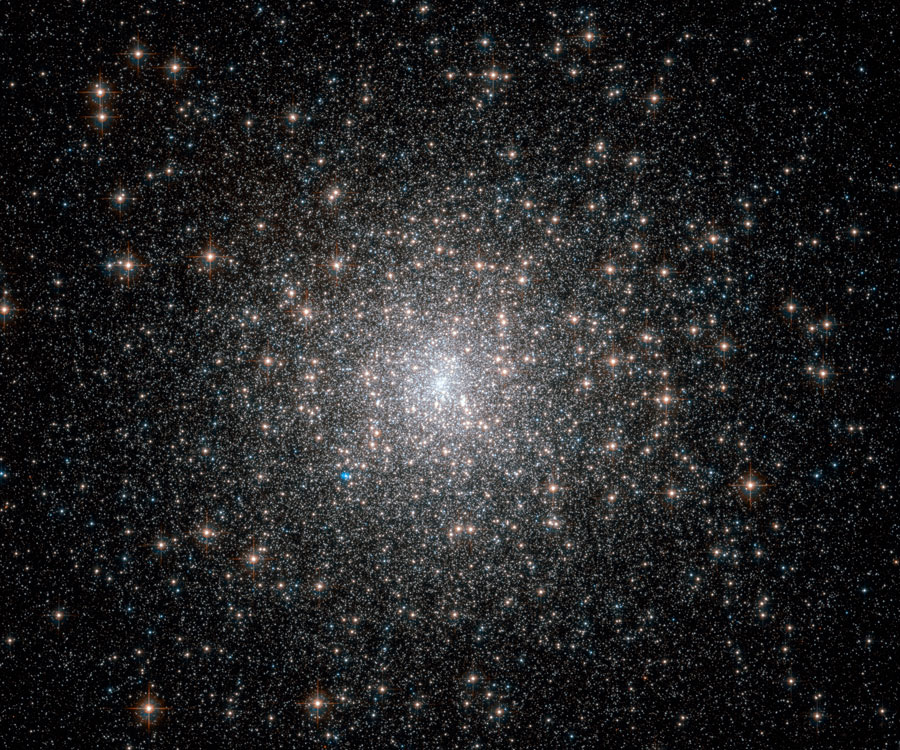
\includegraphics[width=12cm]{images/m15.jpg}
\caption[M15 Globular Cluster]{Globular Cluster M15, taken by the Hubble Space Telescope with an exposition time of 900 seconds. Image by NASA}
\end{figure}

Let's discuss in further the details of these systems.

\subsection{Basics}

A Globular Cluster is a compact, gravitationally bound group of hundreds of thousands to several million stars that are themselves gravitationally bound to galaxies. They have comparable ages to their associated galaxies which is an encouraging characteristic to study them as they could provide valuable information about the formation and evolution of their host galaxies.

Their star populations are uniformly old, although different stellar populations are found as we improve our measurements and observations, such as in the case of the recent study of the stellar populations in the globular clusters of the Fornax dwarf galaxy, where multiple stellar populations and nitrogen abundances have been found (Larsen \& Brodie et- al 2014). Globular clusters are devoid of gas so that pretty much no new stars form in them. The stars at the centre of a globular cluster are much more densely packed than the stars in other parts of the galaxy.

Globular clusters revolve about the nucleus of a galaxy on orbits of high eccentricity and high inclination to the galactic plane. About a third of globular clusters are concentrated around the galactic center. A typical cluster has a period of revolution around the order of $ 10^{8} $ years. A cluster spends most of its time far from the center of a galaxy, and so most of them can, and have been discovered in the spaces between galaxies. 

Due to clusters moving in various orbits in the Galaxy, they are bound together with gravitational forces that are stronger than the disrupting forces exerted on it by the Galaxy or other nearby stars, and this results in an added condition for the stability of a cluster.

The spherical shape of these systems is due to the reached stability that they can acquire over time. To ensure the stability of an isolated cluster, the average speed of its individual stars must not exceed the escape velocity from the cluster. If this occurred, the stars would escape into space, and the cluster would dissipate. If the stellar velocities are low enough to satisfy this condition, then the cluster is gravitationally bound, i.e. the force of gravity is strong enough to keep the member stars from escaping.

Another factor in the stability of clusters is size; the smaller and more compact the cluster, the greater its own gravitational binding force compared with the disrupting forces, and the more chance it has to survive to old age.

Because globular clusters are highly compact systems, they are consequently very stable, and so most globular clusters will probably maintain their identity almost indefinitely. But even these clusters lose some stars, especially if they have a low mass. This is due to there always being a few stars in a cluster that move faster than the cluster's average speed.

When a star escapes, it carries with it energy, removing this energy from the cluster as a whole. This eventually results in the cluster developing a tightly bound core surrounded by a rarefied halo of stars as we can see in the following images of Globular Clusters:

\begin{figure}[H]
\centering
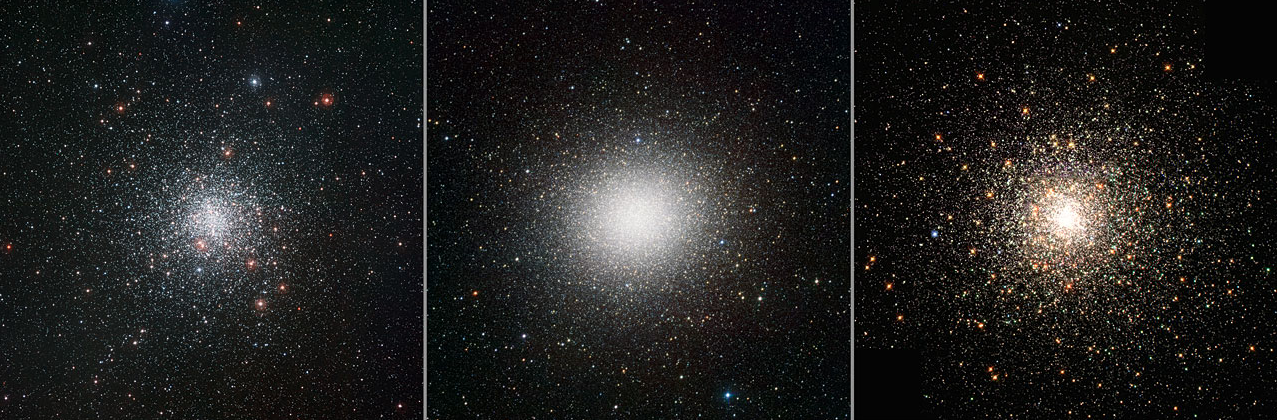
\includegraphics[width=14.5cm]{images/3_gcs.png}
\caption[ESO and Hubble images of Globular Clusters]{Globular Clusters taken by ESO and the HST. From left to right: M4 (ESO), Omega Cen (ESO) and M80 (Hubble). Images from the Hubble Space Telescope database.}
\end{figure}

In the dense core of a cluster, the stars occasionally collide, and some of the debris eventually coalesces. Predictions indicate that this dynamical evolution could lead to the development of a large Black Hole at the cluster's center. At the same time, a few stars in the outer parts of the cluster would continue to escape. The escape rate and dynamical evolution for the rich globular clusters are so slow that the clusters can easily survive for many billions of years, remaining mostly unchanged.

Observations and mass models of these structures show that the average star density in a Globular Cluster is about 0.4 stars per cubic parsec. In the dense center of the cluster, the star density can increase from 100 to 1000 per cubic parsec, as we shall discuss in another section. However, even in the center of clusters, there is still plenty of space between the stars.

In order to understand how dense Globular Clusters can be, we may think of a clear example like Proxima Centauri, which is 4.2 light-years, or about 1.3 parsecs from Earth. Thus, if we were able to draw a sphere around the Sun with a radius of 1.3 parsecs, it would only contain 2 stars: the Sun and Proxima Centauri. But if you were to draw this same sphere in the center of the globular cluster M13, it would contain approximately 10,000 stars.

To summarize and compare some of the main characteristics we just mentioned about globular clusters with other stellar systems let's see the following table:

\begin{table}[H]
\begin{tabular}{| c | c | c | c |}
\hline
\textbf{Characteristic}              & \textbf{Open Custers} & \textbf{OB Associations} & \textbf{Globular Clusters}  \\
\hline
Diameter $ (pc) $ & $<10$ & $30-200$ & $20-100$ \\ \hline
Number of Stars & $50-1000$ & $10-100$ & $10^{4}-10^{6}$ \\ \hline
Mass ($M_{\odot}$) & $100-1000$ & $100-1000$ & $10^{4}-10^{6}$ \\ \hline
Density ($M_{\odot}/pc^{3})$ & $0.1-10$ & $<0.01$ & $0.5-1000$ \\ \hline
Shape & Irregular & Irregular & Spherical \\ \hline
Color (Common) & Red or Blue & Blue & Red \\ \hline
Metallicity & High & High & Low \\ \hline
Location & Disk of Galaxy & Disk of Galaxy & Halo of Galaxy \\
\hline
\end{tabular}
\caption[Summary chart of Star Clusters]{Summary chart of Star Clusters, taken from  http://astronomyonline.org}
\end{table}

\subsection{Formation and evolution}

The formation of Globular Clusters is not well understood yet, and we only have crude ideas of their typical states right after they have reached the dynamical equilibrium.

As it was mentioned in the introduction, two main broad types of possibilities have been considered to explain the very first processes that created these structures. The first one suggests that in the early universe the first structures that came to exist were globular clusters by Jeans Fragmentation. One of the main contributions to this possibility was given by Peebles \& Dicke (1968) who first pointed out that globular clusters might have formed even before the collapse of the protogalaxy, noting the fact that the baryonic Jeans mass right after decoupling is about the size of a Globular Cluster. Although their possibility is in concordance with the current scenario of galaxy formation in which galaxies are formed inside the deepest regions of the gravitational potential well provided by dark matter halos, there are still problems of this theory, for example, it cannot explain why there are so few intergalactic globular clusters and why the properties of globular clusters are correlated with their host galaxies.

Another problem with this theory is some observational results like the ones found by Odenkirchen et al. (2003) who found tidal tails surrounding globular clusters. This is not expected if globular clusters form and reside inside extended dark matter halos that would keep the stability and thus avoiding the creation of these tidal tails.

The second possibility suggests that the formation of Globular clusters was a response to thermal instabilities present in large hot halos of massive galaxies full of gas. In their model, cold dense clouds condense out of hot and tenuous background to form as progenitors of globular clusters. This idea corresponds to the late-forming theory Globular Clusters that could be in accordance with the present observational properties of Globular Clusters like their characteristic metallicity, but it has proven difficulties to justify the assumed thermal behaviour of the cluster-forming gas clouds. Also, there are observations that suggest that very low mass galaxies, not massive enough to host a hot gaseous halo, may also have their own globular clusters.

Many theories on Globular Cluster formation assume a smooth and rapid collapse of the protogalaxy (Eggen, Lynden-Bell, \& Sandage 1962) but some other authors (Searle \& Zinn 1978) state that the early Galactic environment migth have been much more chaotic and violent.

Murray \& Lin (1992) have argued that self-gravitating clouds are unstable to fragmentations and spontaneous star formation so that globular clusters must form from sub-Jeans mass clouds. In subsequent work Murray et al. (1993) have shown that only clouds in a limited mass range ($10^{4}M_\odot\lesssim M\lesssim 10^{6}M_\odot$) can survive both the Kelvin-Helmholtz  instability and the thermal instability which does not lead to bound clusters. Clouds within the critical mass range will form globular clusters if they are induced into cooling and collapse by collisions of sufficient velocity.

Mathews \& Schramm proposed a schematic merger model for the formation of the halo and chemical evolution of the Galaxy in which the protogalaxy forms by mergers of small subgalactic gas clouds. This merger model, as discussed by Lee, Schramm \& Mathews 1994 could also be a possible scenario for Globular Clusters formation. 

Moving on to the evolution of these systems, we note that our current observations and modelling give us good results after the equilibrium has been reached, in this context, there must be mentioned that the mechanism that drives the system to stability is relaxation. This proccess pretty much erases the cluster's memory of it's initial state so the results for gravitational stable systems can be reached using a wide range of initial conditions.

Since the relaxation time is inversely proportional to density evolution due to relaxation proceeds most rapidly in the dense central regions of the clusters. Within this central region that is relaxed, the distribution function $f$ and the density distribution should be approximate to a isothermal distribution, this means that the distribution function must be approximately Maxwellian at energies well bellow the escape energy. We asume that in the outer parts of the clusters the relaxation time is long and encounters have relatively little effect.

Other important characteristic of their evolution is they lose mass from stellar evolution: Our stellar evolution theories show us that stars often eject mass from their surfaces near the ends of their lives. For the mass-losing stars inside globular clusters, the ejected mass is likely to escape the cluster, either because the ejection velocity exceeds the escape speed from the cluster or because it interacts with the galactic gas when the cluster is passing throw the disk. So we conclude that the clusters lose mass as stars evolve. It must be mentioned that the evolution timescale of a typical population of stars is usually much longer than the crossing time in the cluster.

The mass lost by a cluster due to stellar evolution depends on the initial mass function  which specifies the distribution of masses of stars just after they have formed and the initial-final mass function. 

Now, when we talk about the evolution of the Globular Clusters, we must see how the mass distribution evolves over time. the evolution of the mass distribution in an isolated cluster, that began as a Plummer model (that we shall introduce in the following section) is shown in the next figure:

\begin{figure}[H]
\centering
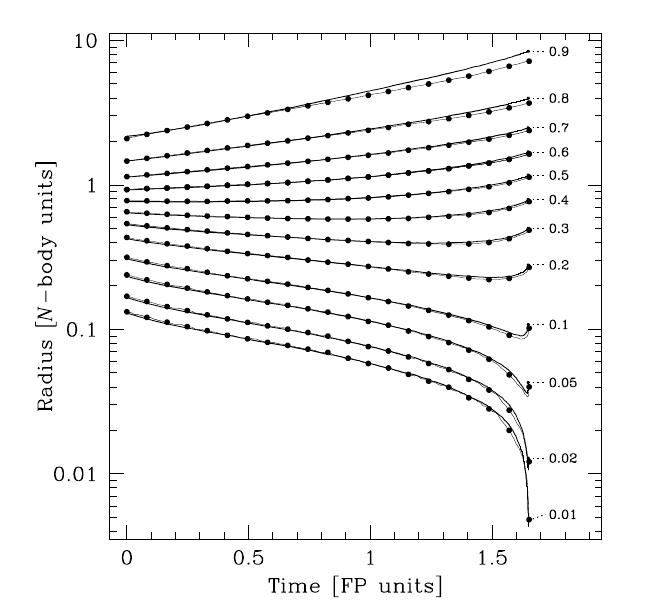
\includegraphics[width=12cm]{images/core_collapse.png}
\caption[Evolution of an ergodic Plummer model over time]{Evolution of an ergodic Plummer model, according to an orbit-averaged Monte-Carlo solution of the Fokker Planck equation with $3\times10^{5}$ superstars (heavy solid lines) and an N-body simulation with $65536$ superstars (dots, connected by solid lines). From Freigat, Rasio, \& Baumgardt (2006)}
\end{figure}

As we can see above, the outer half of the cluster expands, mainly due to the gradual growth of the halo as stars in the core diffuse towards the escape energy. But most importantly, we can see that the center contracts, this process is known as \textbf{core collapse} and it leads to a dramatic growth in the central density that may indicate the existence of an apparent singularity in the central density.

By solving the orbit-averaged Fokker-Planck equation for an isolated, spherical cluster (without binaries) and starting from a Plummer model, Takahashi (1995) found a more accurate calculation of core collapse. His calculations allow greater dynamic range than Monte Carlo or N-body methods. His results show that as the cluster evolves, the core radius shrinks  and the central density grows. Outside the core, the density profile approaches a power law $\rho\varpropto r^{-2.23}$.

Another interesting result regarding the direct solutinos of the orbit-avergaed Fokker Planck equations is the behaviour of the anisotropy parameter $\beta=1-\overline{v_{\theta}^{2}}/\overline{v_{r}^{2}}$ as we can see in the following figure:

\begin{figure}[H]
\centering
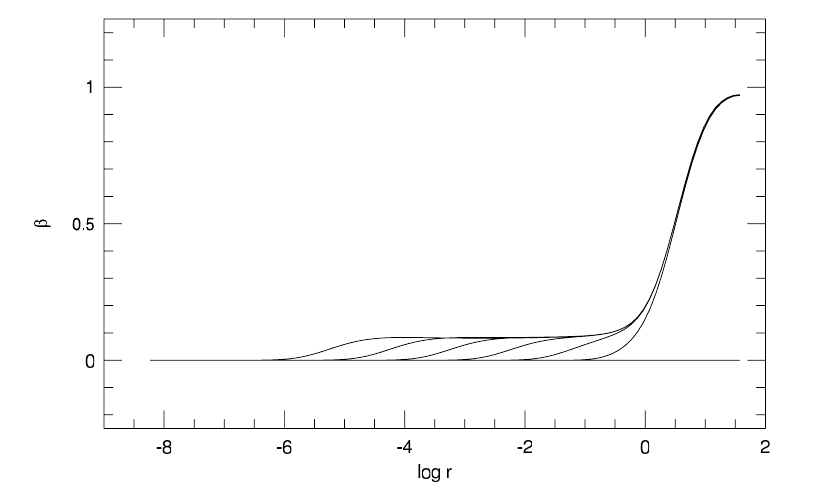
\includegraphics[width=12cm]{images/anisotropy_core_collapse.png}
\caption[Evolution of the velocity anisotropy parameter]{The evolution of the velocity anisotropy parameter for an orbit-averaged Fokker Planck calculation of core collapse. From Takahashi (1995)}
\end{figure}

At large radii, the anisotropy parameter (that indicates the tendency of the system to have or not preferred directions) tends to unity ($\beta\simeq1$), and that indicates that the orbits are nearly radial, at the smalest radii, inside the shrinking core, we have $\beta\simeq0$, which indicates that the velocity distribution is isotropic. We note that in the radius range in which the density profile in the top panel is a power law, there is a constant small radial anisotropy of $\beta\simeq0.08$ or  $\overline{v_{\theta}^{2}}/\overline{v_{r}^{2}}\simeq0.92$. We will discuss the details of these parameters in the next section.

Regarding the late interactions and accretion processes, we note that although our Galaxy has evidently not experienced any further major accretion events capable of disrupting the disk, it is possible that minor accretion events affecting only the halo and not the disk have continued to occur (Navarro, Frenk, \& White 1994), but their net effect on the GC's dynamics and stability is the context of cosmology is very low.

The evolution process for these systems are so long that this fit entirely in the context of Cosmology. Most of the clusters whose masses are larger than $10^{5}M\odot$ have lifetimes longer than the Hubble time.

\subsection{Observational Properties}

Globular clusters were once thought to consist of a single population of stars that all formed together. However, research has since shown that many of the Milky Way's globular clusters had far more complex formation histories and are made up of at least two distinct populations of stars.

A way of analysing the stellar populations in Globular Clusters is to use Colour-Magnitude diagrams. A colour-magnitude diagram is a plot of the apparent magnitudes of the stars in a cluster against their colour indices. Globular Clusters nearly all have very similar colour-magnitude diagrams.

This diagram for a typical globular cluster looks very different than that of an open cluster. There are no Main Sequence stars of types OBAF, but there are many red giants. The brightest stars in a globular cluster are those at the tip of the red giant branch in the color-magnitude diagram, which explains the red appearance of the bright stars in color images of the clusters. You can also see stars populating the horizontal branch (and also why it is called the horizontal branch), the asymptotic giant branch, and even some stars that have colors and magnitudes of F stars, but far fewer than the G stars just below and to the right of them on the Main Sequence. As we can see in the following figure:

\begin{figure}[H]
\centering
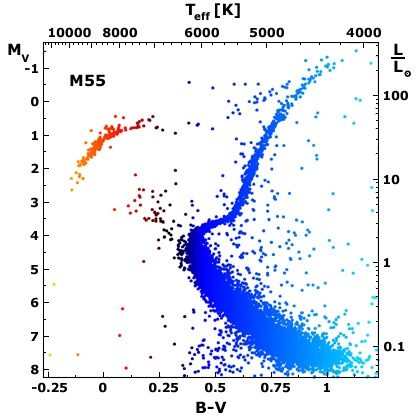
\includegraphics[width=10cm]{images/m55_diagram.jpg}
\caption[Color Magnitude diagram of M55]{Color Magnitude diagram of M55. Image by NASA}
\end{figure}
 
Of these populations, around half the stars are a single generation of normal stars that were thought to form first, and the other half form a second generation of stars, which are polluted with different chemical elements. In particular, the polluted stars contain up to 50–100 times more nitrogen than the first generation of stars.

The proportion of polluted stars found in the Milky Way's globular clusters is much higher than astronomers expected, suggesting that a large chunk of the first-generation star population is missing. A leading explanation for this is that the clusters once contained many more stars, but a large fraction of the first-generation stars were ejected from the cluster at some time in its past.

An interesting plot relating the age of the Globular Clusters to their metallicity is shown in the following figure:

\begin{figure}[H]
\centering
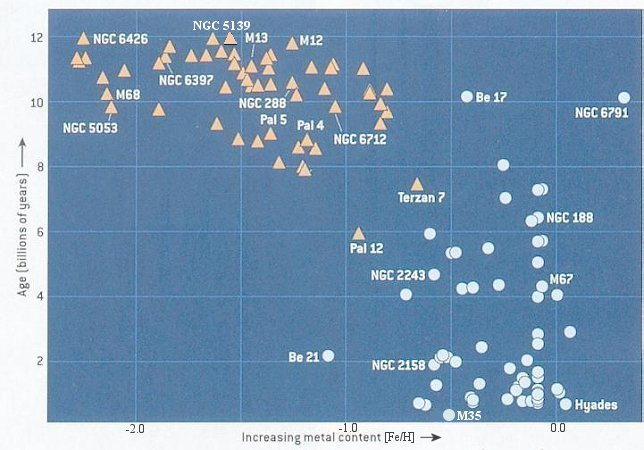
\includegraphics[width=10cm]{images/metallicity_gcs.jpg}
\caption[Age vs Metallicity for some Globular Clusters]{Age estimations vs metallicity of Open (circles) and Globular (triangles) Clusters. Taken from https://universe-review.ca}
\end{figure}

Before now, we didn't know whether globular clusters in smaller galaxies had multiple generations or not, but our observations show clearly that they do. This finding means that a leading theory on how these mixed-generation globular clusters formed cannot be correct, and astronomers will have to think once more about how these mysterious objects in the Milky Way and further afield came to exist.

The other fundamental observational procedures to study GC's are Radial velocity measurements that have revealed that most Globular Clusters are moving in highly excentric elliptical orbits that take them far outside the Milky Way; they form a halo of roughly spherical shape which is highly concentrated to the Galactic Center, but reaches out to a distance of several 100,000 light years, much more than the dimension of the Galaxy's disk. As they don't participate in the Galaxy's disk rotation, they can have high relative velocities of several 100 km/sec with respect to our solar system; this is what shows up in the radial velocity measurements. Ninkovic (1983) has estimated eccentricities of globular cluster orbits. Cudworth and Hanson (1993) undertook some first rough determinations of proper motions with respect to background galaxies. From these and similar measurements, Van den Bergh (1995) estimated perigalactic distances, and Dauphole et.al. (1996) calculated first approximate orbits. Much more acurate data for proper motions became only available from astrometrical data obtained with ESA's Hipparcos satellite in 1997, from which space motions (Geffert et.al. 1997) and approximate orbits (Brosche et.al. 1997) could be determined.

We can visualize their orbits in the following figure:

\begin{figure}[H]
\centering
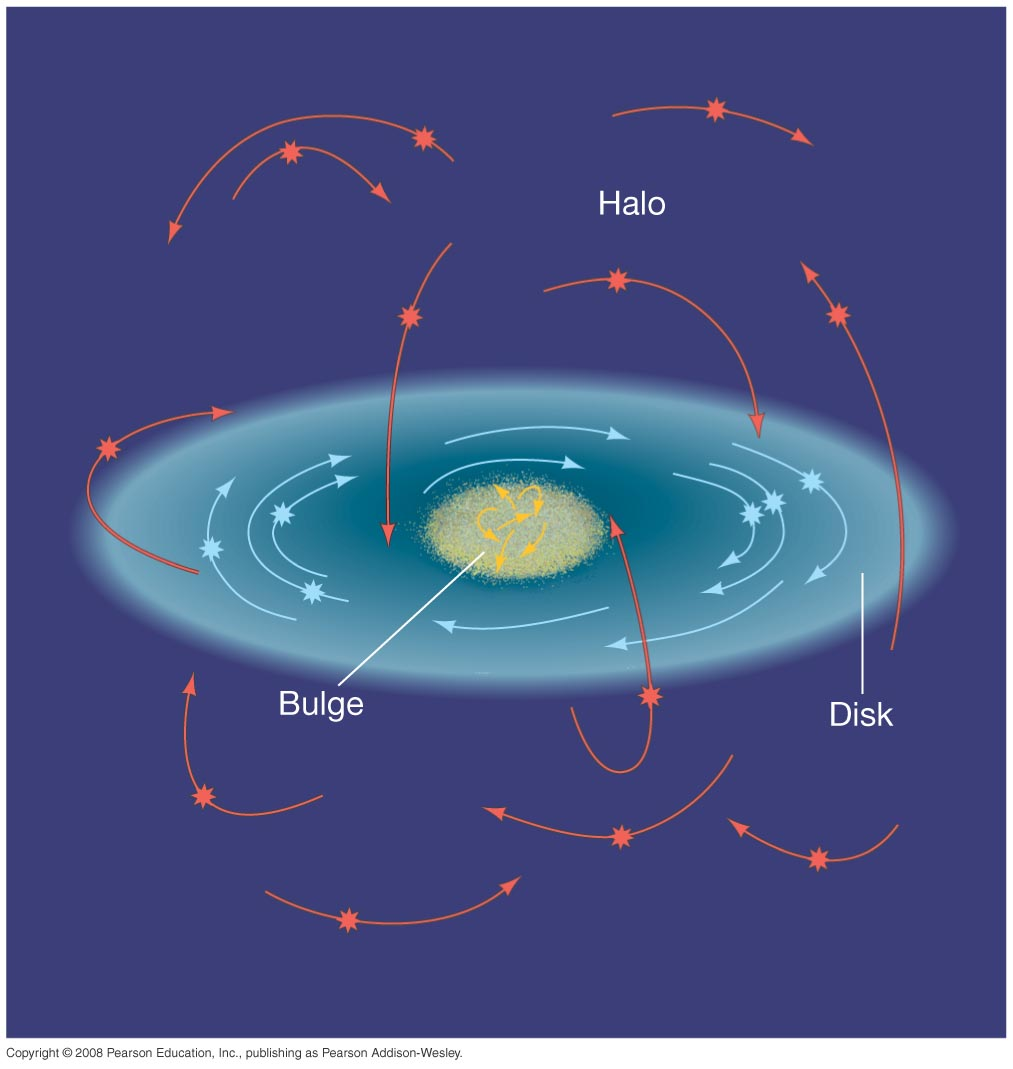
\includegraphics[width=10cm]{images/orbits_gcs.jpg}
\caption[Illustration of the orbits of Globular Clusters around a spiral galaxy]{Illustration of the orbits of some Globular Cluster in a spiral galaxy like the Milky Way. Picture from the Oregon University webpage}
\end{figure}

To determine the physical orbits of stars in globular clusters, it is required to know their proper motions in addition to their radial velocities. This can be achieved by measuring the doppler broadening of the spectral lines in the clusters as we can see in the following figure

\begin{figure}[H]
\centering
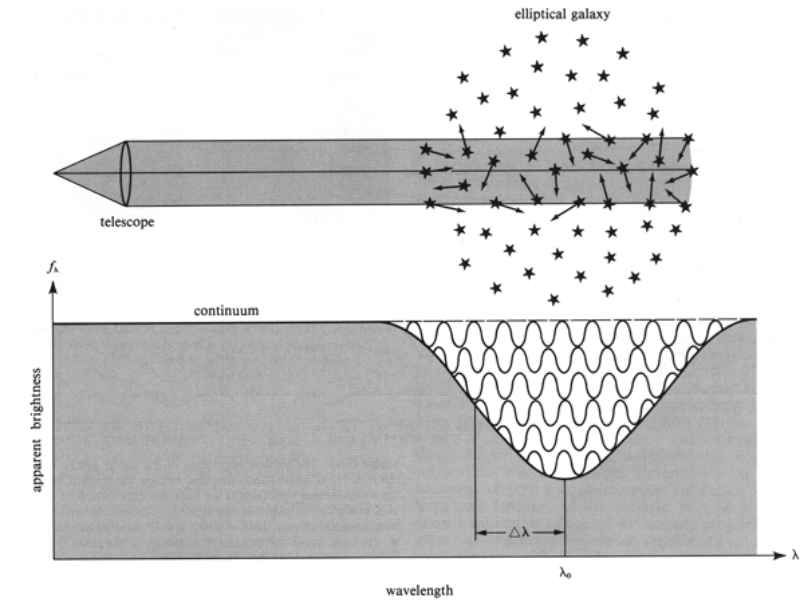
\includegraphics[width=10cm]{images/4_gcs.png}
\caption[Spectral line broadening]{Observed spectral line broadening due to the proper motions of stars in the cluster, note that the observed $\Delta\lambda$ is given by the blue shift or red shift of each individual star contributing to the broadening of the line, this gives important information about the velocity dispersion that will be discussed in a following section. Taken from lecture notes of the University of Arizona}
\end{figure}

We will study further the mass models that fit best to Globular Clusters and the dynamical structure in the following section.

\section{Mass models and Dynamics}

In order to get into the physical discussions about the stability and modelling of globular clusters, we need to understand first the basics of potential theory, and more specifically the potential theory of spherical systems. The next step is to discuss the physical implications behind these models so that the mass modelling can be made. The last but most important part is to discuss the criteria regarding the mathematical treatment of the dynamics of these systems in the context of the collisionless Boltzmann equation and the approximations to the solutions of the Jeans equations that will be used for the fitting of the observational data to do the final modelling.

\subsection{Potential Theory of Spherical Systems}

Our discussions about Potential Theory for large stellar systems will be studied using the simplifications given by the spherical symmetry of globular clusters. We first introduce some of the most important theorems for calculating the gravitational potential of an spherically symmetric distribution of matter provided by Newton, these theorems are physically related to Gauss theorem and may be proved using simple geometric assumptions or using a more precise results from vectorial calculus.

\textbf{Newton's first theorem} states that a body that is inside a spherical shell of matter experiences no net gravitational force from that shell. 

\textbf{Newton's second theorem} states that the gravitational force on a body that lies outside a sphericall shell of matter is the same as it would be if all the shell's matter were concentrated into a point at its center. 

It follows from Newton's theorems that the gravitational attraction of a spherical density distribution $\rho(r')$ on a unit mass at radius $r$ is entirely determined by the mass interior to $r$:

\begin{equation}
\textbf{F}(r)=-\frac{GM(r)}{r^{2}}\hat{\textbf{e}}_{r}
\end{equation}

Where the mass as a function of the radius is

\begin{equation}
M(r)=4\pi\int_{0}^{r}dr'r'^{2}\rho(r')
\end{equation}

We can consider that the total gravitational potential of the spherical system is the sum of the potentials given by spherical shells of a differential mass $dM(r)=4\pi\rho(r)r^{2}dr$. This way, we may calculate the gravitational potential at $\textbf{r}$ generated by a spherically symmetric density distribution $\rho(\textbf{r}')$ by adding the contributions to the potential produced by shells with $r'<r$, and with $r'>r$. Thus we obtain:

\begin{equation}
	\begin{aligned}	
	\Phi(r) &= -\frac{G}{r}\int_{0}^{r}dM(r')-G\int_{r}^{\infty}\frac{dM(r')} {r'}\\      &= -4\pi G\left[\frac{1}{r}\int_{0}^{r}dr'r'^{2}\rho(r')+\int_{r}^{\infty}dr'r'\rho(r')\right]
	\end{aligned}
\end{equation} 

We note an important property of a spherical matter distribution regarding its circular speed $v_{c}(r)$, defined to be the speed of a particle of negligible mass in a circular orbit at radius $r$. We may evaluate $v_{c}$ by equating the gravitational attraction $|\textbf{F}|$  to the centripetal acceleration ${v_{2}}^{2}/r$:

\begin{equation}
v_{c}^{2}=r|\textbf{F}|=r\frac{d\Phi}{dr}=\frac{GM(r)}{r}
\end{equation}

We may also note that the \textbf{escape speed} $v_{e}$ in terms of the gravitational potential is:

\begin{equation}
v_{e}(r)\equiv\sqrt{2|\Phi(r)|}
\end{equation}

The \textbf{potential energy of spherical systems}  comes from a very general equation, also in terms of the potential:

\begin{equation}
W=-\int d^{3}x\rho x\cdot\nabla\Phi
\end{equation}

By substituting equation (2.1) and integrating over all directions of \textbf{r} we get:

\begin{equation}
W=-4\pi G\int_{0}^{\infty}drr\rho(r)M(r)
\end{equation}

The potential energy tensor of a spherical body is \textbf{diagonal} i.e it is isotropic, and has the form:

\begin{equation}
W_{jk}={{1}\over{3}}W\delta_{jk}
\end{equation}

Once we have the general results for the potential of spherical distributions we can move on to study special cases, let's study potential-density pairs that would best fit for Globular Clusters.

The simplest model is the \textbf{homogeneous sphere} of radius $a$, characterized by the gravitational radius $r_{g}\equiv GM^{2}/|W|$, with $r_{g}=\frac{5}{3}a$, for which the gravitational potential is:

\begin{equation}
\Phi(r) = \left\lbrace
\begin{array}{ll}
-2\pi G\rho\left(a^{2}-\frac{1}{3}r^{2}\right) & (r<a)\\
-\frac{4\pi G\rho a^{3}}{3r} & (r>a)
\end{array}
\right.
\end{equation} 

For spherical systems, the density is roughly constant near the center, and falls to zero at large radii. A potential of a system of this type would be proportional to $r^{2} + constant$ at small radii and to $r^{-1}$ at large radii. The \textbf{Plummer Model} is a simple potential with these properties and it it of the form:

\begin{equation}
\Phi=-\frac{GM}{\sqrt{r^{2}+b^{2}}}
\end{equation}

What characterises this model to a simple homogeneous sphere model is the linear scale that generates the potential, which is called the \textbf{Plummer scale length} $b$ while $M$ represents the total mass of the system. From this potential, using spherical coordinates we can calculate $\nabla^{2}$:

\begin{equation}
\nabla^{2}\Phi=\frac{1}{r^{2}}\frac{d}{dr}\left(r^{2}\frac{d\Phi}{dr}\right)=\frac{3GMb^{2}}{\left(r^{2}+b^{2}\right)^{5/2}}
\end{equation}

And from $\nabla^{2}\Phi=4\pi G\rho$ (\textbf{Poisson's equation}) the corresponding density to the potential:

\begin{equation}
\rho(r)=\frac{3M}{4\pi b^{3}}\left(1+\frac{r^{2}}{b^{2}}\right)^{-5/2}
\end{equation}

And finally the potential energy of a Plummer model is:

\begin{equation}
W=-\frac{3\pi GM^{2}}{32b}
\end{equation}

In 1911 Plummer used this potential-density pair to fit observations of Globular Clusters since it gets rid if the indetermination that would arise if we didn't include the Plummer scale length.

Another useful model is given by the \textbf{Isochrone Potential}, that gives analytic orbits to all the stars orbiting the system (For a Plummer potential the position of a star orbiting the system cannot be given in terms of elementary functions). This model is of the form:

\begin{equation}
\Phi(r)=-\frac{GM}{b+\sqrt{b^{2}+r^{2}}}
\end{equation}

By Poisson's equation the density associated with the isochrone potential is:

\begin{equation}
\rho(r)=\frac{1}{4\pi G}\frac{1}{r^{2}}\frac{d}{dr}\left(r^{2}\frac{d\Phi}{dr}\right)=M\left[\frac{3\left(b+a\right)a^{2}-r^{2}(b^{2}+3a)}{4\pi(b+a)^{3}a^{3}}\right]
\end{equation}

So that in the extreme cases the isochrone potential yields:

\begin{equation}
\rho(r) = \left\lbrace
\begin{array}{ll}
\frac{3M}{16\pi b^{3}} & (r=0)\\
\frac{bM}{2\pi r^{4}} & (r\gg b)
\end{array}
\right.
\end{equation} 

As a very useful approximation, we can work with \textbf{Two-power density models}. First, we note that the luminosity density of many elliptical galaxies can be approximated as a power law in radius at both the largest and smallest observable radii, with a smooth transition between these power laws at intermediate radii. Some numerical simulations of the clustering of dark matter particles suggest that the mass density within a dark halo has a similar structure. This is the reason for which much attention has been given to models with a density of the form:

\begin{equation}
\rho(r)=\frac{\rho_{0}}{\left(r/a\right)^{\alpha}\left(1+r/a\right)^{\beta-\alpha}}
\end{equation}

Dark matter halos are often modelled by the above equation with $\beta\simeq3$ and $\alpha$ in the range $(1,1.5)$. Dehnen models are the solutions for $\beta =4$ that have simple analytic properties. But we may discuss some specific results summarized in the following table:

\begin{table}[H]
\begin{center}
  \begin{tabular*}{0.35\textwidth}{@{\extracolsep{\fill} } c  c  c }
    \hline
    \textbf{Model} & $\alpha $ & $\beta $ \\ \hline
    Hernquist (1990) & 1 & 4 \\
    Jaffe (1983) & 2 & 4 \\
    NFW (1995) & 1 & 3 \\
    \hline
  \end{tabular*}
\end{center} 
\caption[Two power density potentials]{Two-power densitiy potentials given by the different values of $\alpha$ and $\beta$}
\end{table}

Navarro, Frenk, \& White (1996) showed that the values taken by the free parameters $\alpha$ and $\beta$ for the halos that formed in their simulations were strongly correlated, so the halos were essentially members of a one-parameter family. 

According to equation (2.17) the mass inside the radius $r$ is:

\begin{equation}
M(r)=4\pi \rho_{0}a^{3}\int_{0}^{r/a}ds\frac{s^{2-\alpha}}{(1+s)^{\beta-\alpha}}
\end{equation}

For the important cases we discuss, the mass is

\begin{equation}
M(r) = 4\pi \rho_{0}a^{3} \times \left\lbrace
\begin{array}{lll}
\frac{r/a}{1+r/a} & \text{for a Jaffe model}\\
\frac{(r/a)^{2}}{2(1+r/a)^{2}} & \text{for a Hernquist model}\\
ln(1+r/a)-\frac{r/a}{1+r/a} & \text{for a NFW model}
\end{array}
\right.
\end{equation} 

We can directly integrate the mass to get the potential for the three discussed models:

\begin{equation}
\Phi(r) = -4\pi G\rho_{0}a^{2} \times \left\lbrace
\begin{array}{lll}
ln(1+r/a) & \text{for a Jaffe model}\\
\frac{1}{2(1+r/a)} & \text{for a Hernquist model}\\
\frac{ln(1+r/a)}{r/a} & \text{for a NFW model}
\end{array}
\right.
\end{equation} 

From the above equations, and taking into account the potential energy for each model, it can be proved that the Jaffe and Hernquist models have gravitational radii $r_{r}=2a$ and $6a$ respectively, while for the NFW model $r_{g}$ is undefined. The circular speed, given by these potentials for each model is shown in the following figure: 

\begin{figure}[H]
\centering
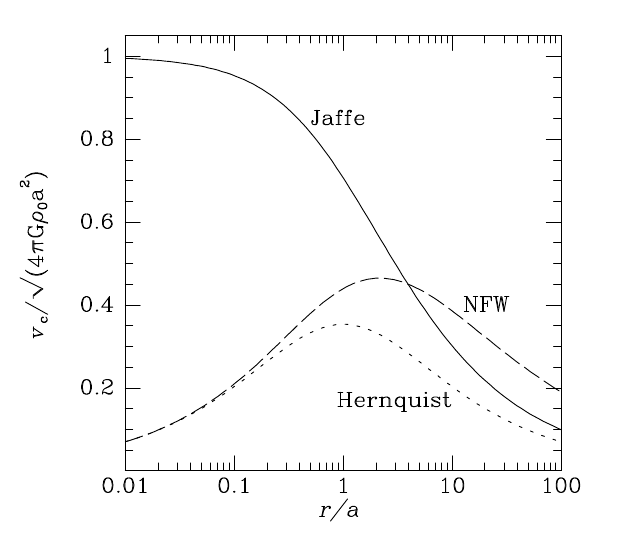
\includegraphics[width=10cm]{images/circular_velocity_vs_radius.png}
\caption[Circular speed vs radius for the Jaffe, Hernquist, and NFW models]{Circular speed vs radius for the models of Jaffe, Hernquist and NFW, taken from Binney \& Tremaine, Galactic Dynamics 2$^{nd}$ edition.}
\end{figure}

The next step in the analysis of the dynamics and stability of Globular Clusters is to understand the physics of spherical distribution of systems and how the solutions for their dynamics can be easily reached. As we shall see, a good consideration for the simplification of the mathematical treatment of Globular Clusters (with good physical reasons) is that these systems are not collisional.

\subsection{Collisionless Systems}

The problem of modelling the structure and dynamics of Globular Clusters is not trivial whatsoever. Several assumptions and physical approaches need to be made to simplify the problem and reach results that fit the observational data. One of the main assumptions is that the stellar systems that we will study are \textbf{collisionless}. This assumption not only reduces the problem of determining the functional form of the position and velocities of the stars but also has strong physical reasons that must be mentioned.

In the context of stellar systems, collision refers to any interaction between individual particles, such as direct encounters, gravitational assistance, sudden disruption of the orbit, or any interaction that changes the stars orbit in a significant way. That the system is collisionless means that it is a system in which the interaction cross-section between particles (stars in this case) is so low that collisions between particles have no significant effect on the system so that the dominant component of the dynamics is the potential well produced by the system as a whole.  

One of the other approximations we make is that the orbits of stars in the system can be determined by assuming that the mass of the Globular Cluster is distributed smoothly in space, rather than concentrated in certain positions as point masses. The true orbits deviate significantly from this approximated model, but in systems with more than a few thousand stars like a globular cluster (that can easily reach hundreds of thousands or millions of stars), the deviation is small and the potential and mass distribution can be approximate as continuous functions. 

As a star moves through a stellar system, it will feel the gravitational force due to all other stars. We want to determine if the motion of the stars is mainly determined by the average gravitational force of all other stars combined, or if it is mostly sensitive to the force due to near stars, in order to do this we must refer to some parameters of time that we properly define like \textbf{relaxation} and \textbf{crossing} time. 

Relaxation usually means the return of a perturbed system into equilibrium. In the clusters, stellar encounters eventually lead to dynamical relaxation, until we say that the system is in a thermal equilibrium. 

The crossing time refers to the typical time that would take to a star to cross the whole system, in terms of the size of the system $r$ and the velocity $v$ of the stars, this time is:

\begin{equation}
t_{cross}=\frac{r}{v}
\end{equation}

The relaxation time in terms of the crossing time and the number of stars $N$ is:

\begin{equation}
t_{relax}=\frac{N}{8ln(N)}t_{cr}
\end{equation}

As these quantities parametrize the interactions between stars, their values really give us a strong idea on how the dynamics can be modelled, as it was mentioned before, for a typical Globular Cluster, the evolution time $t_{evo}$ is usually much larger than the relaxing time which is much larger than the crossing time, so the effects of the interaction between stars is minimal and we can use the approximation that the system is collisionless.

\begin{equation}
t_{cross}\ll t_{relax}\ll t_{evo}
\end{equation}

\subsection{Dynamics}

Using the approximations we just mentioned, the dynamics of stars in Globular Systems can be solved assuming that the those stars are moving under a smooth potential $\phi (x,y,z,t)$ and that at any time $t$ a full description of the state of these systems is given by specifying a function of the number of stars with their position and velocities $f(x,y,z,v_{x},v_{y},v_{z},t)$ or $f(\vec{\textbf{x}},\vec{\textbf{v}},t)$ which is called the distribution function of phase space density because it is given in the phase space. This function is the number of stars in volume $d\vec{x}$ with velocities in range $d\vec{v}$ (centered on $\vec{x},\vec{v}$).

This flow of points (or stars) of $f$ is incompressible in the phase space (the density remains conserved along a flow-line) so that

\begin{equation}
\frac{df}{dt}=0
\end{equation}

To infer properly the equation above and understand the time evolution, we define a coordinate $\vec{w}$ for the stars in phase space:

\begin{equation}
\vec{w}\equiv (\vec{x},\vec{v})\equiv (w_{1},w_{2},...w_{6})
\end{equation}

The flow of the star is given by 

\begin{equation}
\dot{\vec{w}}= (\dot{\vec{x}},\dot{\vec{v}})=(\vec{v},-\vec{\nabla} \Phi)
\end{equation}

The flow $\dot{\vec{v}}$ conserves stars so we have the continuity equation:

\begin{equation}
\frac{\partial f}{\partial t}+\sum_{\alpha=1}^{6}\frac{\partial (f\dot{w}_{\alpha})}{\partial w_{\alpha}}=0
\end{equation}

Using the chain rule for $w$ our continuity equation explicitily in terms of the position and velicities is:

\begin{equation}
\frac{\partial f}{\partial t}+\sum_{i=1}^{3}\frac{\partial f}{\partial x_{i}}\dot{x_{i}}+\sum_{i=1}^{3}\frac{\partial f}{\partial v_{i}}\dot{v_{i}}=0
\end{equation}

It is more useful to use the derivative of the velocity in terms of the potential with the relation $\dot{v_{i}}=-\partial\phi / \partial x_{i}$ as:

\begin{equation}
\frac{\partial f}{\partial t}+\sum_{i=1}^{3}\frac{\partial f}{\partial x_{i}}v_{i}-\sum_{i=1}^{3}\frac{\partial f}{\partial v_{i}}\frac{\partial\phi}{\partial x_{i}}=0
\end{equation}

or

\begin{equation}
\frac{\partial f}{\partial t}+\nabla f\cdot\vec{v}-\frac{\partial f}{\partial\overrightarrow{v}}\cdot\nabla\phi=0
\end{equation}

These equations are the Collisionless Boltzmann Equations (CEB) and they are sufficient to calculate the evolution of any distribution function $f$ with time. As the CBE is a very complicated equation of 7 variables, its solution is a challenging task and some assumptions and creative methods have been developed for its solutions, one of them refers to the moments of the distribution function and the other is based on the Jeans theorem.

The moments approximation consists of considering that if the dependence of the phase space density upon velocity is relatively smooth and free of singularities, one can collapse the 6-dimensional phase space density into a set of functions of 3-dimensional position by taking moments of the velocities. First, let's note that the moment of order $j$ of the distribution $f$ is

\begin{equation}
\overline{x^{j}}=\frac {\int x^{j}fdx}{\int fdx}
\end{equation}

We can define functions for the characterization of the distribution function on terms of one of its variables:

\begin{equation}
\nu(\vec{\textbf{x}})\equiv \int f(\vec{\textbf{x}},\vec{\textbf{v}})d^{3}v\quad\quad or \quad\quad  \xi(\vec{\textbf{x}})\equiv \int f(\vec{\textbf{x}},\vec{\textbf{v}})d^{3}x
\end{equation}

So that the zeroth moment of the velocity is just the number density $\nu(\vec{\textbf{x}})$ and for each of three velocity components the first moment gives a mean velocity:

\begin{equation}
\bar{v_{i}}(\vec{\textbf{x}})\equiv \frac{1}{\nu(\vec{\textbf{x}})}\int v_{i}f(\vec{\textbf{x}},\vec{\textbf{v}})d^{3}\vec{v}
\end{equation}

Likewise, we can define higher order moments with combinations of powers of the three velocity components. The second moments give a really important and useful quantity related to the \textbf{velocity dispersion tensor} $\sigma^{2}_{ij}$

\begin{equation}
\overline{v_{i}v_{j}}(\vec{\textbf{x}})\equiv \frac{1}{\nu(\vec{\textbf{x}})}\int v_{i}v_{j}f(\vec{\textbf{x}},\vec{\textbf{v}})d^{3}\vec{v}=\sigma^{2}
_{ij}+\bar{v_{i}}\bar{v_{j}}
\end{equation}

The velocity dispersion tensor which will be fundamental in the mass modelling is thus defined as:

\begin{equation}
\sigma_{ij}^{2}=\overline{v_{i}v_{j}}-\overline{v_{i}}\:\overline{v_{j}}
\end{equation}

There is quite some observational support that ideally the velocity distribution functions are reasonably well described by the low order moments; a density and a set of low order moments may therefore give a reasonably complete description of a galaxy or a Globular Cluster. 

Now to find the Jeans equations and show a different approach for the solution of the CBE we need to manipulate the results for the moments of the DF. By multiplying the CBE by powers of the velocity components, and integrating over velocity space we obtain a series of differential equations for the various velocity components on the zeroth moment, we have (using Einstein's notation of summation):

\begin{equation}
\int \frac{\partial f}{\partial t}d^{3}\vec{v}+ \int v_{i}\frac{\partial f}{\partial x_{i}} d^{3}\vec{v}- \frac{\partial\Phi}{\partial x_{i}}\int \frac{\partial f}{\partial v_{}i} d^{3}\vec{v}= 0
\end{equation}

Using the divergence theorem for the last term and replacing by the definitions of $\nu(x)$ and $\overline{v}_{i}\nu(x)$ we get:

\begin{equation}
\frac{\partial}{\partial t}\nu+\frac{\partial}{\partial x_{i}}(\nu \overline{v}_{i})=0
\end{equation}

Which looks just like a standard 3-D continuity equation. Now, we do the same procedure for the first moment, (again taking the spatial and temporal derivatives outside the velocity integrals) and integrating by pats and expressing the results in terms of our average velocities:

\begin{equation}
\frac{\partial}{\partial t}(\nu \overline{v}_{j})+\frac{\partial}{\partial x_{i}}(\nu \overline{v_{i}v_{j}})+\frac{\partial \Phi}{\partial x_{i}}\int f\frac{\partial v_{j}}{\partial v_{i}}d^{3}\vec{v}=0
\end{equation} 

The last term on the left hand side becomes $\nu \delta_{ij}$ in an orthogonal coordinate system. So applying the product rule and our continuity equation to the first term we get

\begin{equation}
\nu \frac{\partial \overline{v}_{j}}{\partial t}-\overline{v}_{j}\frac{\partial}{\partial x_{i}}(\nu \overline{v}_{j})+\frac{\partial}{\partial x_{i}}[\nu(\sigma_{ij}^{2}+\overline{v}_{i}\overline{v}_{j})]=-\nu \overline{v}_{i}\frac{\partial \Phi}{\partial x_{j}}
\end{equation}

Where we used the relation between the second moments and the velocity dispersion, finally differentiating the second term on the left hand side, part of the result cancels part of the third term and we arrive to the \textbf{Jeans' equations} for a collisionless fluid

\begin{equation}
\begin{aligned}	
	\nu \frac{\partial \overline{v}_j}{\partial t} + \overline{v}_i\nu \frac{\partial\overline{v}_j}{\partial x_{i}} &= -\nu \frac{\partial\Phi}{\partial x_{j}}-\frac{\partial}{\partial x_{i}}(\nu \sigma_{ij}^{2})\quad\quad (j=1,2,3) \\     acceleration + viscosity &= gravity + pressure
	\end{aligned}
\end{equation}

One important use of the Jeans' equations is to calculate the number density and potential self-consistently, assuming
a given model for the velocity dispersion.

The Jeans theorem states that any steady state solution of the CBE depends on the phase-space coordinates $(x,v)$ only through integrals of motion in a static potential, and any function of the integrals yields a steady state solution of the CBE. The value of this theorem is that it gives us a way of closing the loop for solving the Boltzmann equation. 

Finally, it is important to introduce a useful parameter called the \textbf{Anisotropy parameter} $\beta$ which gives us information about the preferred directions of the stars in the system, if there are any. In spherical coordinates the anisotropy parameter is

\begin{equation}
\beta=1-\frac{\left(\sigma_{\theta}^{2}+\sigma_{\phi}^{2}\right)}{2\sigma_{r}^{2}}
\end{equation}

If $\beta=0$, then $\overline{v}_{r}^{2}=\overline{v}_{\phi}^{2}=\overline{v}_{\theta}^{2}$ and we have zero anisotropy (there are no preferred directions for the stars in the system and the velocity dispersion tensor is completely symmetric) as in the ideal case of a spherical system in equilibrium. On the other hand, when $\beta=1$ we have that the system has total anisotropy.

\section{Scenario and Observations}

Globular Clusters are relatively easy to observe because they are close to us in the galactic context, for this reason, they have been observed even since the 17th century. The first globular cluster discovered, but then taken for a nebula, was M22 in Sagittarius, which was probably discovered by Abraham Ihle in 1665. This discovery was followed by that of southern Omega Centauri (NGC5139) by Edmond Halley in 1677, which is the largest known globular cluster in our galaxy. This ``nebula" had been known but classified as star since ancient times. Next followed the discovery of M5 in Serpens Caput by Gottfried Kirch in 1702, and that of M13 in Hercules, again by Halley, in 1714. De Chéseaux's list of (21) nebulae of 1746 contains, in addition, two new globular clusters, M71 and M4, while Jean-Dominique Maraldi discovered M15 and M2 in September of this year (1746). Guillaume Legentil possibly or probably discovered NGC 6712 in 1749. Nicholas Louis de Lacaille's catalog of (42) southern "nebula" of 1751-52 contains 8 globular clusters (among them 5 new ones), while Messier's catalog of 110 objects contains a total of 29 "globulars", 20 of them new discoveries. Charles Messier was the first to resolve one globular cluster, M4, but still referred to the other 28 of these objects in his catalog as "round nebulae". Thus, in summer 1782, before William Herschel started his comprehensive deep sky survey with large telescopes, there were 34 globular clusters known. Herschel himself discovered 36 new ``globulars", bringing the number of known ``globulars" to 70. He was the first to resolve virtually all of them into stars, and coined the term "globular cluster" in the discussion adjacent to his second catalog of 1000 deepsky objects (1789).

Currently, there are about 150 confirmed Globular Clusters in the Milky Way and the number is growing since we are perfecting our techniques to find globular clusters that may by passing through the disk and thus are complicated to observe.

One important development in recent years is some debated observational evidence that dense, massive star clusters are currently forming in certain environments. It has been suggested that these objects are young globular clusters. This idea is not universally accepted, both because current observations are not definitive and possibly because the notion of young globular clusters flies in the face of the traditional view of globular clusters as ancient objects. However, if globular clusters are forming at the present epoch, we will have the opportunity to study the formation process directly. It seems inevitable that this will greatly enhance our understanding of how and why globular clusters form, as well as deepening our knowledge of the galaxy formation process to which globular cluster formation is intimately related.

Some other observational results of GCs in other galaxies just broadens the current scenario of formation and evolution, for example, in November, 2014 Tim Stephens from the University of California studied some images taken by the HST of four globular clusters located in the small galaxy Fornax to study their properties and compare them with GCs in the Milky Way. What these observations show is that the GCs in the dwarf galaxy Fornax are very similar to our GCs and so they must have formed in a similar way, however, these findings don't fit with the leading theories that have been developed to explain how globular clusters form.   

\begin{figure}[H]
  \centering
  \begin{minipage}[b]{0.45\textwidth}
    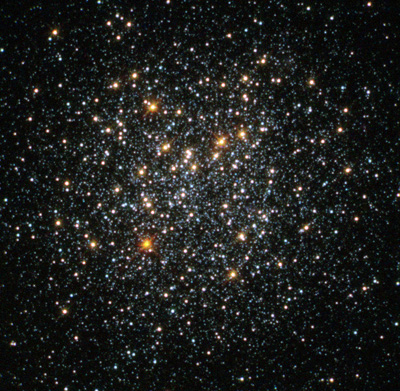
\includegraphics[width=\textwidth]{images/fornax-2-400.jpg}
    \caption[Hubble image of Fornax-2 Globular Cluster]{Image of Fornax-2 Globular Cluster taken by the Hubble Space Telescope. From University of California newscenter.}
  \end{minipage}
  \hfill
  \begin{minipage}[b]{0.45\textwidth}
    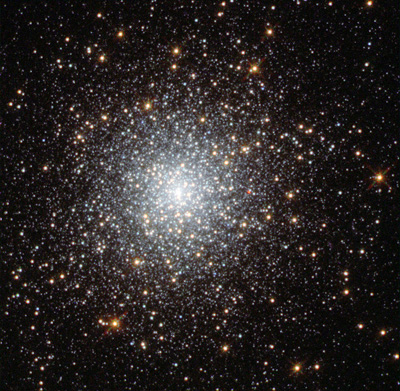
\includegraphics[width=\textwidth]{images/fornax-3-400.jpg}
    \caption[Hubble Space Telescope image of Fornax-3 Globular Cluster]{Hubble Space Telescope image of Fornax-2 Globular Cluster. From University of California newscenter.}
  \end{minipage}
\end{figure}

As mentioned before, Globular clusters in the Milky Way are mainly made up of at least two distinct populations of stars, around half the stars are a single generation of normal stars thought to have formed first, and the other half is a second generation of stars that are enriched with different chemical elements. The proportion of nitrogen-rich stars in the Milky Way's GCs is higher than astronomers expected. This suggests that a large chunk of the first-generation star population is missing. One fair explanation that astronomers have adopted is that clusters once contained many more stars but a large fraction of the first-generation stars were ejected from the cluster at some time in its past. In our galaxy, these stars could go to the halo.

Now, the observations of the Globular Cluster in Fornax contradict this hypothesis since they have found that the proportion of second-generation stars is quite similar to that of the GCs in the Milky Way, but unlike our galaxy, Fornax doesn't have enough old stars to account for the huge number that would have been banished from the clusters, and we should be abe to see them but we don't.

These types of findings mean that a leading theory on how these mixed-generation globular clusters formed cannot be correct and astronomers will have to reconsider how these mysterious objects, in the Milky Way and further afield, came to exist.

In the current scenario, there is  widespread belief that globular clusters cannot contain large amounts of dark matter, because of the Virial Theorem. This theorem relates the velocity dispersion $ \sigma $ that we introduced before at the center of the cluster to the total mass $M_{t}$ and to the half-mass radius $r_{h}$ of the system. For a one component globular cluster, that relation may be expresed as:

\begin{equation}
\left\langle \sigma^{2}\right\rangle \approx0.4\frac{GM_{t}}{r_{h}}
\end{equation}

However, if a dark component is also present, in the form of low-mass objects for example, the virial theorem must be modified to:

\begin{equation}
\sum_{i}M_{t}(i)\left\langle \sigma^{2}\right\rangle _{i}=E_{p}
\end{equation}

Where the index $i$ refers to the different stellar species, and $E_{p}$ is the potential energy of the cluster.

The observational data and mass modelling is still being debated in this manner since the presence of dark matter in the clusters is still a mystery and further work (precisely including the effects of the stellar populations) needs to be done to clarify the scenario and give us a stronger idea on how these objects and galaxies form. 

\section{Simulations}

Efforts are under way by several groups to produce more realistic simulations that properly include the effects of star formation, but the existing results suggest that the first star formation may occur in gas that has become highly condensed at the centers of the first dark-matter halos to form; even though such systems may not closely resemble most present-day galaxies, they may still be of interest as the possible birth sites of globular clusters, as will be discussed further below. The most realistic simulations of the formation of a spiral galaxy like our own have been made by Katz (1992) and Steinmetz \& Muller (1994, 1995), who have simulated the evolution of a spherical galaxy-sized piece of a standard "cold dark matter" universe which is arbitrarily given the appropriate amount of angular momentum. The results show an initial chaotic stage during which mergers between clumps build up a dark halo and a stellar spheroid, followed by a period during which the remaining gas organizes itself into a disk. During the initial chaotic stage several small satellites are formed by the condensation of gas in peripheral dark-matter clumps, and these satellites may survive for a few
orbits before being disrupted and merged into the forming galaxy. It is plausible that such small satellites could be the birth sites of globular clusters, as in the hypothesis of Searle (1977) and Searle \& Zinn (1978) that the globular clusters in the outer halo of our Galaxy were formed in protogalactic ‘fragments’ which survived for a time as independent star-forming systems before being merged to build up the halo

In several earlier reviews of globular cluster chronology, it was concluded that the globular clusters in our Galaxy are not all coeval and that age differences of several Gyr exist in at least a few well-studied cases (e.g., Larson 1990a, 1992b). This conclusion still appears to be valid, and it is supported by the most recent discussion of this subject by Chaboyer, Demarque, \& Sarajedini (1996), which is based on new age estimates for 43 globular clusters

\begin{figure}[H]
\centering
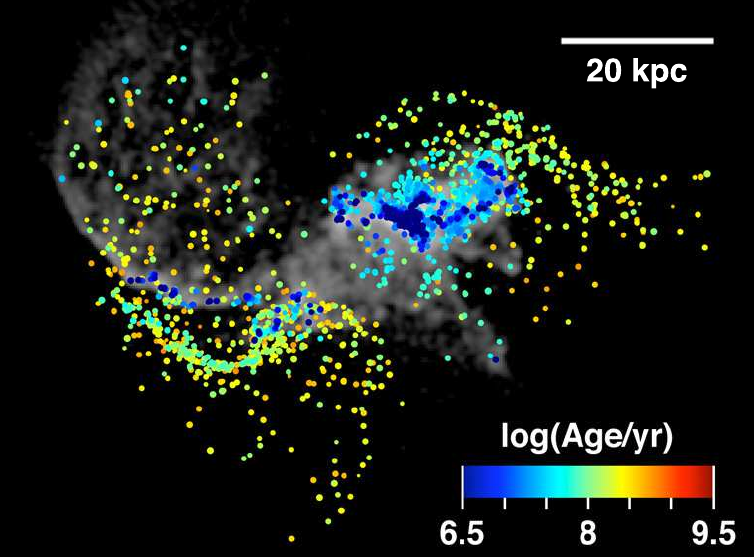
\includegraphics[width=10cm]{images/merger.png}
\caption[Galaxy merger model 1m11 from Kruijssen et al. (2012b)]{Snapshot of galaxy merger model 1m11 from Kruijssen et al. (2012b), which includes a sub-grid model for the formation and evolution of the stellar cluster population. SHown is a merger of two Milky Way-mass galaxies at the time of their first encounter. Coloured dots represent stellar clusters, clour-coded by their ages as indicated by the legend. The grey scale indicates the gas surface density. The snapshot shows how intermediate-age clusters are escaping into the halo, whereas those clusters that formed during the merger reside in the gas-rich, disruptive environment of the discs. This cluster migration process is also seen in observations of nearby galaxy mergers (Bastian et al. 2009).}
\end{figure} % Theoretical Framework 

\lhead{\emph{Obervational Procedures}}
%\usepackage{subfig}

\chapter{Observations and Analysis}

In order to study this problem about the dynamics of Globular Clusters in our galaxy we need scientific data that allows us to build a model that fits our observations. Under supervision of proffesor Juan Carlos Mu\~noz Cuartas and with three other undergraduate students from the University of Antioquia a trip to the OPD (Pico dos Dias Observatory) was made to Brazil in May 2014, besides the observational experience of the students, the main purpose of the trip was to get important data for this project. We needed two sets of data corresponding to spectra and photometric images of the Globular Clusters

The spectroscopic data allows us to determine the velocity dispersion profile in the inner region of globular clusters while the photometric data allows us to study the surface brightness distribution for them. We can use all of this information to infer the properties of the globular clusters' mass distribution in order to build complete dynamical models and therefore infer the amount of dark matter present in the globular clusters (if there is any).

\section{Observational Procedures}

Our stay in OPD consisted of two days in the main dome for the spectroscopic data (using the Perkin-Elmer (P\&E) telescope with a 1.6m mirror and the Cassegrain Spectrograph) and four days in a smaller dome for the photometric data in the IAG telescope with a 0.6m mirror. In the following photograph, the domes of the observatory that we used for our observations:

\begin{figure}[h]
\centering
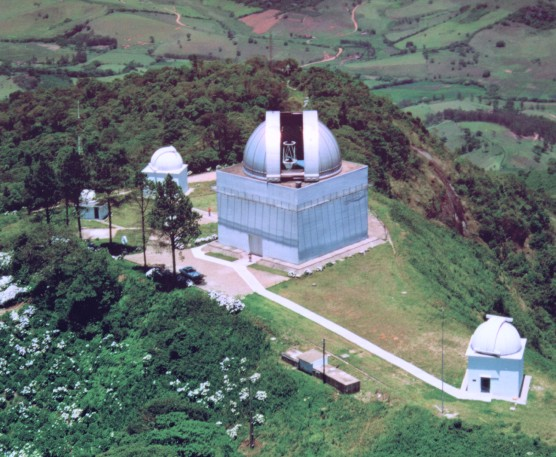
\includegraphics[width=10cm]{images/opd.jpg}
\caption{OPD observatory seen from the air, the big dome was used for the spectroscopic data and the small dome at the low right part of the photo for the photometric data.}
\end{figure}

\subsection{Spectroscopic Data}

The first two days (May 14th and 15th) we took the spectroscopic data in the telescope P\&E with a diameter of 1.6m. The main instrument was the Cassegrain spectrograph with a CCD Ikon-L camera and Filters BVR. The software we used was the recently installed software TCSPD which is built in a LabView environment for Windows (2010). Here's a photo of the telescope from inside the dome:

\begin{figure}[h]
\centering
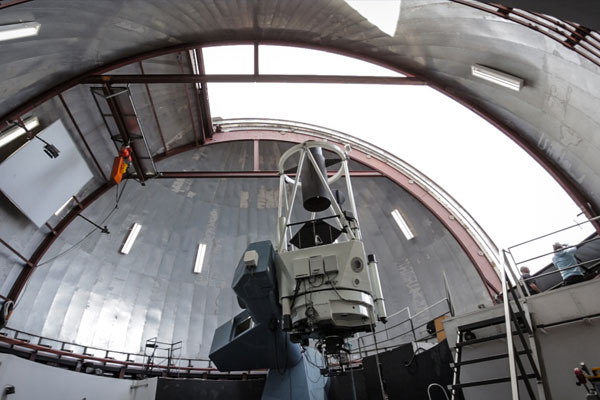
\includegraphics[width=10cm]{images/opd-spectrograph.jpg}
\caption{Perkin-Elmer telescope in the main dome in OPD used for the spectroscopic observations}
\end{figure}

We made the observations of dome flats, bias frames, comparison lamp frames, calibration stars and certain globular clusters of the milky Way organized by the best observation times using Simbad and Stellarium for the estimations of the coordinates and times respectively. We needed to keep an order of the observations to make the most of our observation time in OPD so we decided to organize our Globular Clusters in different groups or "chunks":

\begin{figure}[h]
\centering
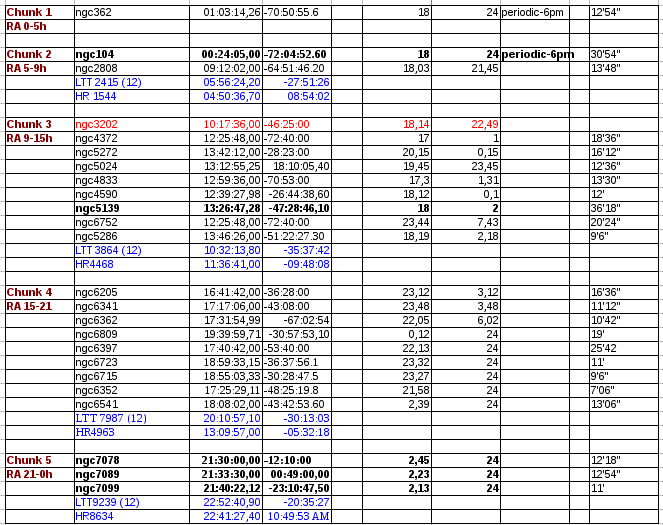
\includegraphics[width=10cm]{images/9.png}
\caption{Organized globular Clusters in groups for the proper times}
\end{figure}

Now, our set up configuration for the spectrograph was the following:

On May 14th, a diffraction grating of 900 lines per mm, a CCD IkonL and the central wavelength for the observations of 8500 Angstroms (with possibility of rotation of the slit 90°, +45° and -45°).we used the slit of 2.52" and obtained data for the globular clusters: NGC-5020, NGC-5272, NGC-4833, NGC-4590, NGC-5139, NGC-5286, NGC-6752, NGC-6397, NGC-6723, NGC-6715 and NGC-6541 using exposition times of 600 and 900 seconds. We also observed the calibration stars: HR-4963 and HR-4468 with 7 and 5 seconds. As it was the first day, we needed to be very careful in calibrating our instruments on order to have the objects in the right focus, we also made the rotation of the slit to use all the diffraction angles of the observations and our comparison lamps were of Ne-Ar.

On May 15th, we used the slit of 3.0", and used a central wavelength of 5500 Angstroms. This time we observed the following objects: NGC-2802, NGC-5024, NGC-4590, NGC-5139, NGC-5286, NGC-5272, NGC-6362, NGC-6397, NGC-6723, NGC-6502, NGC-6541, NGC-7078, NGC-7099, the stars HR-4468 and HR-7950 and we also observed Mars for pedagogical reasons. We used pretty much the same exposition times than the day before, this time though, our comparison lamps were or He-Ar. All the data we took was in FITS format (Flexible Image Transfer System).

\subsection{Photometric Data}

The photometric data were acquired in the next four days (from May 16th to May 19th) in the 0.6m IAG telescope in OPD. We used the Johnson system for the different filters which were easily shifted with the given software in the control computers. Here a picture of the telescope from inside the dome:

\begin{figure}[h]
\centering
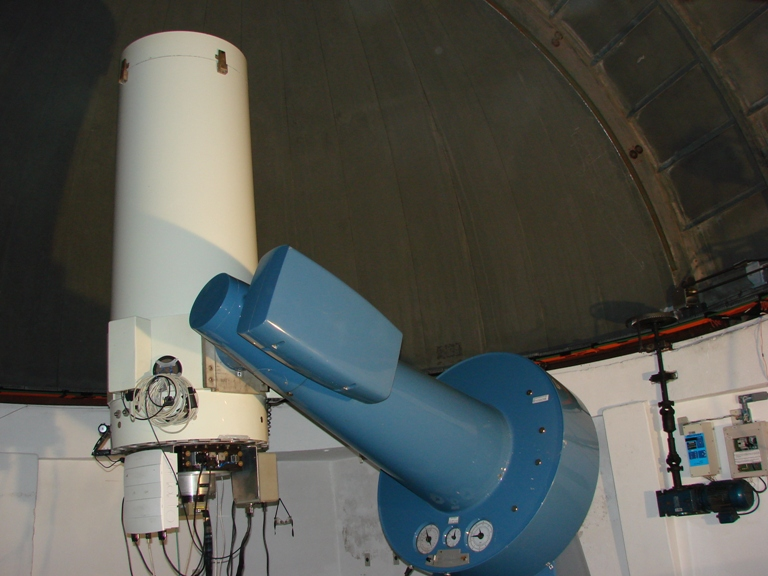
\includegraphics[width=8cm]{images/opd-photometry.jpg}
\caption{IAG telescope used for the photometric data}
\end{figure}

On May 16th, we took all the calibration images, consisting of 20 bias frames with an exposition time of 0,00001 seconds; also 22, 11, 11, 20 and 10 flat frames for the B,I,R,U,V filters respectively, their exposition times differed, for  U filter we took various frames of 60 and 30 seconds, for the B filter we took frames of 30 seconds each, 15s for I, 60s for R and 3s for V. We took our "focus" images to calibrate the instrument, and also various skyflats for all the filters. We targeted the following globular clusters and calibration stars in different filters: NGC5272, HR4961, NGC4590, NGC5139 AND NGC6397. The exposition time for the clusters was of 600 seconds and 2 and 4 seconds for the calibration star. 

May 17th was a terrible night for observations because the sky was too cloudy and the only useful data we could get were dome flats for the filters I,R and V that we could use instead of the bad dome flats of the first day. The reduction using the flats of another day are decent but this is not the ideal situation since mechanical movements of the instrument might slightly change its configuration and therefore it probably ends up with a reduction that is not the ideal one for science purposes.  

On May 18th we were more organized since we were getting familiar with the observations and therefore the data we got had little trouble in the upcoming analysis, even though the sky was clody at the end of the night. The science objects we observed were NGC5139, HR6308, NGC6723, NGC6541, NGC7078, HR7964 that were observed in the different filters. We got 20 bias frames, 14 dome flats in the vaious filters, but no skyflats. 

On May 19th we observed the Globular Clusters NGC5139, NGC4590, NGC6723, NGC6715, NGC6541, NGC6970, NGC5286, NGC639, NGC6541 and NGC6715, the calibration stars HR6386 and HR6386, 20 bias frames and flats for each filter.

\section{First step for Anaysis}

Our first goal in starting the analysis of all the relevant data was to organize all the images in order to reduce the time required to make the reductions. For every day the calibrations images, trash, calibration stars and objects were separated and they were given their correct names as they were in the headers and compared with the information sheets we filled at the time we were doing the observations. With the use of an account on the galaxy.udea.edu.co cluster, for proper and quicker analysis and safety of the data, all the files were correctly organized.

The next step was the reduction of all the images with the calibration files for each day, I started the photometric data to acquire certain skills in the use of IRAF because the reduction of the spectroscopic data was to be a little more complex and needed a deeper understanding of IRAF packages. 

I started with the cluster NGC-5139 ($ \Omega $ Centauri) because we got lots of data for that cluster in OPD and also because $ \Omega $ Centauri is a well known globular cluster since it is the largest in our galaxy and we can get a lot of information from the web. 

After the photometry of that cluster, the most relevant part of the reduction was to be made. The reduction and analysis of the spectroscopic data (May 14th and 15th), the methods for these reductions are quite special and are the most relevant part of the analysis because that is our most valuable information. The reduction was to be made very carefully because a good spectroscopic analysis depends upon a good reduction of the data. Just as with the photometric data, the first procedures were made for the Cluster NGC5139 to understand and master the techniques of the reduction and extractions.

\section{Photometry}

The photometry was made by the two traditional methods, PSF photometry and Aperture Photometry; even though the magnitudes calculated using both methods are quite different, the calibration constant between the two methods gave a good relation between them and made me trust the photometry results.

But first, the reduction of the data had to be done. The first step is to characterize the calibration images in order to see if there are any errors associated with the instrument or the way that the observations were made. By doing this we found that most of the flat-field images had brightness gradients in the corners and this was a problem we needed to correct because the increased value on the counts in these corners would affect the normalization of the super-flat that we would use to reduce the science data. Another systematic error that we found in all of our calibration and science frames was the prescence of a strange water-looking figure at the top left corner of them, although it can be removed with the correct reduction, it obviously affected the CCD sensitivity by the time of the observations. Also, some filters showed a higher sensitivity to this systematic errors but at the end, the photometry could be made in the best data so that the dirty images don't affect our results.

In order to see how the data would be affected by the systematic errors we just mentioned, we produced a composite image using three images with the filters U,V and R and we did the same with the flats in those filters, the resultas are shown in the following figure:
  
\begin{figure}[h]
  \centering
  \begin{minipage}[b]{0.45\textwidth}
    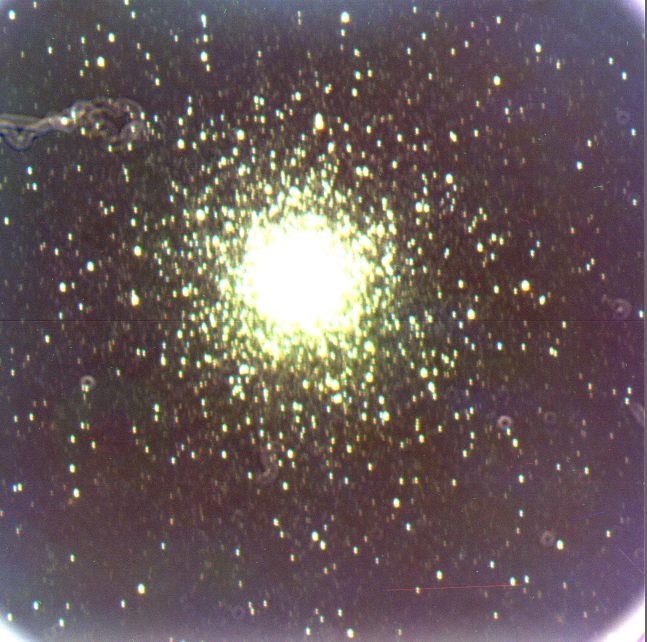
\includegraphics[width=\textwidth]{images/ngc_5139_dirty.png}
    \caption{Composite image of NGC5139 without being previously reduced}
  \end{minipage}
  \hfill
  \begin{minipage}[b]{0.45\textwidth}
    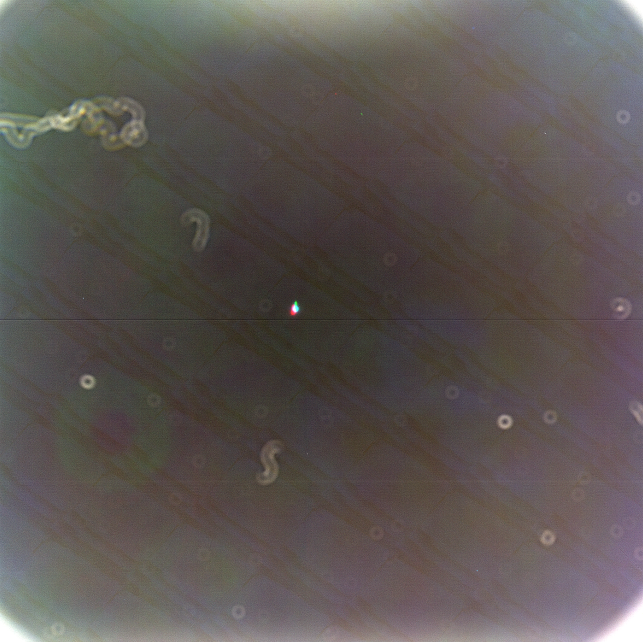
\includegraphics[width=\textwidth]{images/ruido.png}
    \caption{Composite image of the flats showing the noise that needs to be extracted}
  \end{minipage}
\end{figure}

What we can infer from these images is that the flat fields and the bias frames contain the same noise that the science data thus giving us a good result in the reduction.

Once all the characterization is made we can reduce our important data using IRAF following the conventional steps consisting of: 

building a super-bias

Hago un Superbias a partir de los bias que tenga
Le resto ese Superbias a todos los flats
Hago un Superflat para cada filtro
A esos superflats los divido por la media de cada uno
Las imágenes originales las divido por esos flats

\begin{figure}[h]
\centering
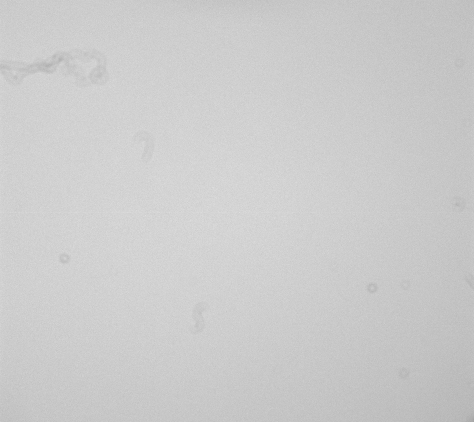
\includegraphics[width=8cm]{images/flat_I.png}
\caption{Normalized Superflat for the I filter}
\end{figure}




Photometry using Phot

\section{Spectroscopy}


\subsection{Spectroscopic Reduction}

- First we make a Superbias combining all the bias frames and then we subtract it from all the lamp, targets and flat field frames.

- It was important to analize the flats to see which ones are saturated, we consider that values over 65,000 counts (using implot) show saturated data. The ones that we could trust for May 14th were ten images called flats\_0012 to flats\_0021.

- The pre-superflat is made using the median given the number of images.

- We need to make a trimming in all images because there are some regions in the images that show unexpected luminosity, this is probably due to border errors in the camera or the obturator time of relaxation. The zones we decided to cut were:

[0-100] and [575 to the end]

- A critical step is the creation of a response function, this is made by collapsing the pre-superflat to one column using blkavg. The useful image for the creation of the Superflat is done by combining this column with blkrep. This gives us an image that's uniformly distributed in the dispersion axis with the following IRAF commands.

blkavg MasterFlat.fits[1:475,*] AvgFlatCols 475 1

blkrep AvgFlatCols AvgFlatColsMaster 475 1

- The pre-superflat is now divided by the response function we created (AvgFlatColsMaster) and this gives us the Superflat that we will use to reduce our data.

- Finally, the task we use to remove the cosmic rays is lacos, and it gives very accurate results, as it shows the "mask" image with the removed cosmic rays.

\subsection{Extraction}

Once the reduction is ready, we can proceed with the extraction of the spectra of the calibration stars and also the spectra of the stars in the clusters, this procedure is made with the task apall.

Taking special care of correctly choosing the background, and with the following parameter configuration:

b\_number: 100

background: fit

weight: vairance

saturate: 65215

rdnoise: 6

gain: 1

Interactively, one must choose very precisely the background regions to extract the spectrum and do the fitting routines with different orders until the best results are reached.

The extraction of the spectrum for the calibration lamps is done with apsum, which is very similar to apall.

\subsection{Wavelength Calibration}

The wavelength calibration is made many tasks of IRAF like Identify, Refspec and Dispcor. First, with identify I use the interactive window in IRAF to select some prominent lines in the spectrum and assign them their correct wavelength using the theoretic spectrum of the lamp. In this case our calibration lamps were Ne-Ar (for May 14th) and He-Ar (for May 15th)  and OPD observatory provided us the theoretic distribution of emission lines of them.

Using "m" to select the larger lines and typing the wavelength, the task creates a file stored in a new folder "database" with the pixels with their corresponding values in units of Angstroms. After that, the targets were to be calibrated with these files so it is necessary to edit their header to assign them the reference frames. It is enough to change the REFSPEC1 image header on each lamp file in order to do the wavelength calibration. 

The task that actually does the calibration on wavelength is dispcor, it is only necessary to run the task over all the targets with their own calibrated arc to get the calibrated spectrum which is the useful and important file to make the analysis of the width of the lines and their redshift.

\subsection{Flux Calibration}

The aim is to calibrate the CCD chip response, spectrograph+telescope throughput and allow for atmospheric extinction. The result is a spectrum as observed from outside the atmosphere with an ideal uniformly sensitive detector+telescope+spectrograph. Basically, what the flux calibration does is, it takes from a tabular compilation the energy distribution of the standard star, it corrects this energy distribution for wavelength-dependent atmospheric extinction, it compares it to the energy distribution of the observed spectrum and derives from such a comparison the function that gives the response of our system for every wavelength.

The flux calibration takes place in three parts: Calibrating from the standard star, calculating the sensitivity function of the instrument, and finally, applying the calibration to the spectra. We will use the task observatory to determine observatory parameters, standard to flux calibrate each standard star, and sensfunc to finally determine the wavelength response and the solution will be applied to the spectra by the task calibrate.

In the first part, the calibration is made with one of the stars that are already included in IRAF, there are many stars so there's quite a good amount of options to choose. So the first task is the task standard. The observatory parameter is specified as LNA which is in IRAF's database. 

\textbf{The task standard}

The task standard determines calibration pass-bands and writes them to a file called std. The thrick here is to specify the location of the the input extinction and flux calibration files. To do that, I edit the parameters of standard with the following routes:

Extinction file:                              onedstds\$/ctioextindt.dat

Directory containing calibration data:   onedstds\$ctionewcal/

Starname in calibration list:                l9239

Where I chose the Star l9239 because it has the spectral range that we use in our calibration Stars. And running the task interactively would be enough for this step.

\textbf{The task sensfunc}

Standard task just recorded response of each standard star so the next step is to put the results together and find a proper wavelength dependence of instrumental sensitivity and atmosphere transparency using the task sensfunc. It creates an image with a default name sens.0001. IRAF needs to have some general idea of atmospheric extinction before to start, so I set again extinct onedstds\$ /ctioextinct.dat.

Now, running the task interactively and taking into account that the function used to fit the instrumental response will be usually of very high order. A good idea is to use spline3 fitting (:function spline3) with some 20 pieces, i.e. (:order 20).
Finally q exists the sensfunc task and writes the sens.0001 image.

\textbf{The task calibrate}

The solution to each star to be calibrated is done with the task calibrate. Editting the parameters of calibrate to set the appropriate extinction table: extinct onedstds\$ /ctioextinct.dat would be enough for this purpose. The task is run over all the wavelength calibrated spectra which had their airmass and other parameters appropriately set by the eso.set procedure. And finally it gives the flux-calibrated spectra ready for the relevant analysis concerning radial velocities.

After the flux calibration, I notice that the extremes of the spectra have irregularities but that can be cut because they don't have any relevant information.

For the star calibration I cut from 0 to 45 and from 1860 to the end, using imcopy:

\begin{center}
imcopy flux\_calib\_star\_fits[45:1860,*] cut\_flux\_calib\_star.fits
\end{center}

In order to normalize the spectrum, first I find the maximum value in the spectrum using minmax and then I divide the whole image by this value.

Now, to create the Ascii table from the spectrum I need to first convert my image to a 1D image using the task scopy and setting format=onedspec

Now, with the image ready in 1D, I use the task wspectext to create the Ascii table like this:

\begin{center}
wspectext ready\_flux\_star.0001.fits normal\_cut\_flux\_star\_calib.txt
\end{center}

\section{RVSAO and radial velocity determination} % Observational Procedures
 
\lhead{\emph{Modelling}} 
\chapter{Modelling}

We used various techniques for the determination of the dynamic and stellar mass of NGC5139 that we use to model the mass more accurately. 


\section{Modified Hernquist Model}

Four experiments:

Density profile

\begin{equation}
\rho(r)=\frac{M}{2\pi}\frac{a}{r}\frac{1}{\left(r+a\right)^{3}}
\end{equation}

Cumulative mass

\begin{equation}
M(r)=M\frac{r^{2}}{(r+a)^{2}}
\end{equation}
 
Surface brightness 
 
 \begin{equation}
 I(R)=\frac{M}{2\pi a^{2}\Gamma\left(1-s^{2}\right)^{2}}\left[\left(2+s^{2}\right)X(s)-3\right]
 \end{equation}
 
 where $s=R/a$, $R$ is the projected radius and:

\begin{equation}
X(s)=\frac{1}{\sqrt{1-s^{2}}}sech^{-1}s\qquad for\qquad0\leq s\leq1
\end{equation}

\begin{equation}
X(s)=\frac{1}{\sqrt{s^{2}-1}}sec^{-1}s\qquad for\qquad1\leq s<\infty
\end{equation}

For computational simplicity we have written some of the trigonometric functions just like Hernquist did: $sec^{-1}s = cos^{-1}(1/s)$ and $sech^{-1} = ln[(1+\sqrt{1-s^{2}})/s]$

Line of sight velocity dispersion

 \begin{equation}
 I(R)\sigma_{p}^{2}(R)=\frac{2}{\Gamma}\int_{R}^{\infty}\left(1-\beta\frac{R^{2}}{r^{2}}\right)\frac{\rho\bar{v_{r}^{2}}rdr}{\sqrt{r^{2}-R^{2}}}
 \end{equation}

Now, for the velocity dispersion we have:

\begin{equation}
\bar{v_{r}^{2}}=\sigma_{r}^{2}=\frac{1}{\rho(r)}\int_{r}^{\infty}\rho(r)\frac{d\phi}{dr}dr
\end{equation}

Where 

\begin{equation}
\frac{d\phi}{dr}=\frac{GM(r)}{r^{2}}
\end{equation}

So the projected velocity dispersion becomes:

\begin{equation}
\sigma_{p}^{2}(R)=\frac{2}{I(R)\Gamma}\int_{R}^{\infty}\left(1-\beta\frac{R^{2}}{r^{2}}\right)\left(G\int_{r}^{\infty}\frac{\rho(r)M(r)}{r^{2}}dr\right)\frac{rdr}{\sqrt{r^{2}-R^{2}}}
\end{equation}

We do various experiments and fits for our modelling, first, the simplest of all models is the one where we assume that the cluster doesn't have dark matter whatsoever, in this case there only will be one mass contribution and only one scalength (the stellar scalength) then the solution of the last equation would be:

\begin{equation}
\sigma_{p}^{2}(R)=\frac{GM^{2}a}{I(R)\Gamma\pi}\int_{R}^{\infty}\alpha(r)\left(\frac{\log{\left(\frac{a+r}{r}\right)}}{a^{5}}-\frac{25a^{3}+52a^{2}r+42ar^{2}+12r^{3}}{12a^{4}\left(a+r\right)^{4}}\right)dr
\end{equation}

Where $a$ is the scalength and where, in order to shorten the equation we take $\alpha(r)$ as 

\begin{equation}
\alpha(r)=\left(1-\beta\frac{R^{2}}{r^{2}}\right)\frac{r}{\sqrt{r^{2}-R^{2}}}
\end{equation}

Now, as we want to focus on the dark matter content of the cluster, we assume that the mass of the cluster is the sum of the mass of stars and the mass of non-baryonic matter so that their contributions to the density and mass profiles become:

\begin{equation}
\rho(r)=\rho_{\star}(r)+\rho_{dm}(r)\qquad and \qquad M(r)=M_{s}(r)+M_{dm}(r)
\end{equation} 

In this case, the projected velocity dispersion takes a much more complicated form as follows:

\begin{equation}
\begin{aligned}	
\sigma_{p}^{2}(R) &= \frac{G}{I(R)\Gamma\pi}\int_{R}^{\infty}\alpha(r)\Biggl[\underbrace{\int_{r}^{\infty}\frac{M_{s}^{2}a_{s}dr}{r\left(r+a_{s}\right)^{5}}}_{\mathbf{A}(r)}+\underbrace{\int_{r}^{\infty}\frac{M_{s}M_{dm}a_{s}dr}{r\left(r+a_{s}\right)^{3}\left(r+a_{dm}\right)^{2}}}_{\mathbf{B}(r)}\right\\      &\left +\underbrace{\int_{r}^{\infty}\frac{M_{dm}M_{s}a_{dm}dr}{r\left(r+a_{dm}\right)^{3}\left(r+a_{s}\right)^{2}}}_{\mathbf{C}(r)}+\underbrace{\int_{r}^{\infty}\frac{M_{dm}^{2}a_{dm}dr}{r\left(r+a_{dm}\right)^{5}}}_{\mathbf{D}(r)}\Biggr] dr
\end{aligned}
\end{equation}

The functional form of the density involves the use of a stellar scalength ($a_{s}$) and a dark matter scalength ($a_{dm}$), Now, the integrals $\mathbf{A}(r),\mathbf{B}(r),\mathbf{C}(r)$ and $\mathbf{D}(r)$ have the following analytical solutions:

\begin{equation}
\textbf{A}(r)=a_{s}\left(-\frac{25a_{s}^{3}+52a_{s}^{2}r+42a_{s}r^{2}+12r^{3}}{12a_{s}^{4}\left(a_{s}+r\right)^{4}}+\frac{\log{\left[\frac{a_{s}+r}{r}\right]}}{a_{s}^{5}}\right)
\end{equation}

\begin{equation}
\textbf{D}(r)=a_{dm}\left(-\frac{25a_{dm}^{3}+52a_{dm}^{2}r+42a_{dm}r^{2}+12r^{3}}{12a_{dm}^{4}\left(a_{dm}+r\right)^{4}}+\frac{\log{\left[\frac{a_{dm}+r}{r}\right]}}{a_{dm}^{5}}\right)
\end{equation}

\begin{equation}
\textbf{B}(r)=\frac{\left(M_{s}M_{dm}\right)\left(\mathbf{b_{2}}+\mathbf{b_{3}}+a_{s}\left(-\left(a_{s}-a_{dm}\right)a_{dm}\mathbf{b_{4}}+\mathbf{b_{5}}\right)\right)}{\mathbf{b_{1}}}
\end{equation}

\begin{equation}
With \left\lbrace
\begin{array}{lllll}
\mathbf{b_{1}}=2a_{s}^{2}(a_{s}-a_{dm})^{4}a_{dm}^{2}(a_{s}+r)^{2}(a_{dm}+r)\\
\mathbf{b_{2}}=-2\left(a_{s}-a_{dm}\right)^{4}\left(a_{s}+r\right)^{2}\left(a_{dm}+r\right)\log{r}\\
\mathbf{b_{3}}=2a_{dm}^{2}\left(6a_{s}^{2}-4a_{s}a_{dm}+a_{dm}^{2}\right)
\left(a_{s}+r\right)^{2}\left(a_{dm}+r\right)\log{[a_{s}+r]}\\
\begin{aligned}	
\mathbf{b_{4}} &= 2a_{s}^{4}+4a_{s}^{3}r-2a_{dm}r(a_{dm}+r)+3a_{s}a_{dm}\left(-a_{dm}^{2}+a_{dm}r+2r^{2}\right)\\      &+a_{s}^{2}\left(7a_{dm}^{2}+7a_{dm}r+2r^{2}\right)
\end{aligned}\\
\mathbf{b_{5}}=2a_{s}^{2}\left(a_{s}-4a_{dm}\right)\left(a_{s}+r\right)^{2}\left(a_{dm}+r\right)\log{[a_{dm}+r]}
\end{array}
\right.
\end{equation} 

\begin{equation}
\textbf{C}(r)=\frac{\left(M_{dm}M_{s}\right)\left(\mathbf{c_{2}}+\mathbf{c_{3}}+a_{dm}\left(-\left(a_{dm}-a_{s}\right)a_{s}\mathbf{c_{4}}+\mathbf{c_{5}}\right)\right)}{\mathbf{c_{1}}}
\end{equation}

\begin{equation}
With \left\lbrace
\begin{array}{lllll}
\mathbf{c_{1}}=2a_{dm}^{2}(a_{dm}-a_{s})^{4}a_{s}^{2}(a_{dm}+r)^{2}(a_{s}+r)\\
\mathbf{c_{2}}=-2\left(a_{dm}-a_{s}\right)^{4}\left(a_{dm}+r\right)^{2}\left(a_{s}+r\right)\log{r}\\
\mathbf{c_{3}}=2a_{s}^{2}\left(6a_{dm}^{2}-4a_{dm}a_{s}+a_{s}^{2}\right)\left(a_{dm}+r\right)^{2}
\left(a_{s}+r\right)\log{[a_{dm}+r]}\\
\begin{aligned}	
\mathbf{c_{4}} &= 2a_{dm}^{4}+4a_{dm}^{3}r-2a_{s}r(a_{s}+r)+3a_{dm}a_{s}\left(-a_{s}^{2}+a_{s}r+2r^{2}\right)\\      &+a_{dm}^{2}\left(7a_{s}^{2}+7a_{s}r+2r^{2}\right)
\end{aligned}\\
\mathbf{c_{5}} =2a_{dm}^{2}\left(a_{dm}-4a_{s}\right)\left(a_{dm}+r\right)^{2}\left(a_{s}+r\right)\log{[a_{s}+r]}
\end{array}
\right.
\end{equation} 

All data (decir los papers de donde salieron todos estos datos)

\begin{figure}[H]
\centering
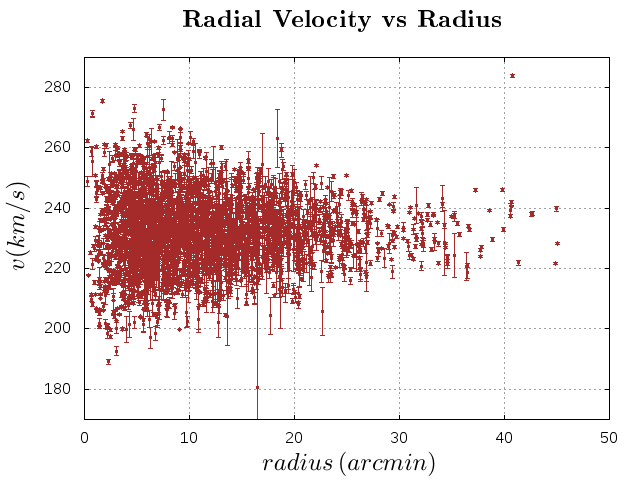
\includegraphics[width=12cm]{images/vel_vs_rad.png}
\caption[Pg]{Pd}
\end{figure}

Error calculation:

Because all the databases provided the associated error to the measurements of the radial velocities, we had to make the proper calculation of the error of the velocity dispersion:

The velocity dispersion is (as mentioned before) the standard deviation of the velocity

\begin{equation}
\sigma = f(v) = \sqrt{\frac{\sum_{i=1}^{n}\left(v_{i}-v\right)^{2}}{N}}
\end{equation}

For our purpose it is calculated in radial bins. 

\begin{figure}[H]
\centering
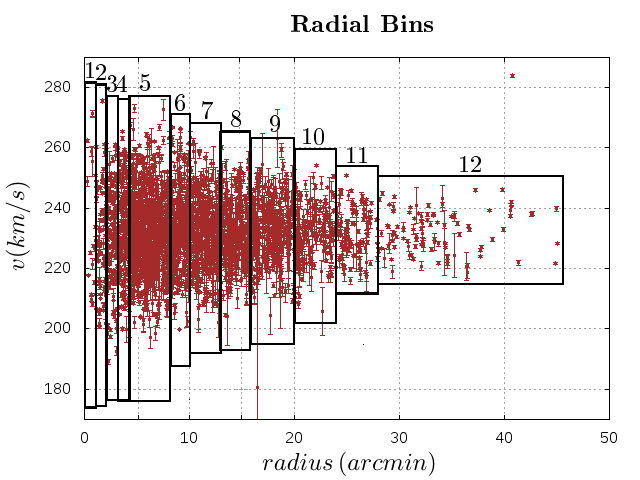
\includegraphics[width=12cm]{images/vel_vs_rad_bins.png}
\caption[Pg]{Pd}
\end{figure}

The error associated with this measurements can be easily calculated using the general error propagation formula:

\begin{equation}
\sigma(v\pm\Delta v)\approx \sigma(v)\pm \underbrace{\frac{\partial \sigma}{\partial v}\Delta v}_{\Delta \sigma}
\end{equation}

\begin{equation}
\Delta \sigma = \frac{1}{\sqrt{N}}\left(\sum_{i=1}^{n}\left(v_{i}-v\right)^{2}\right)^{-1/2}\sum_{i=1}^{n}\left(v_{i}-v\right)\Delta v
\end{equation}



\subsection{Full Modelling}

\textbf{All parameters 12}

\begin{figure}[H]
\centering
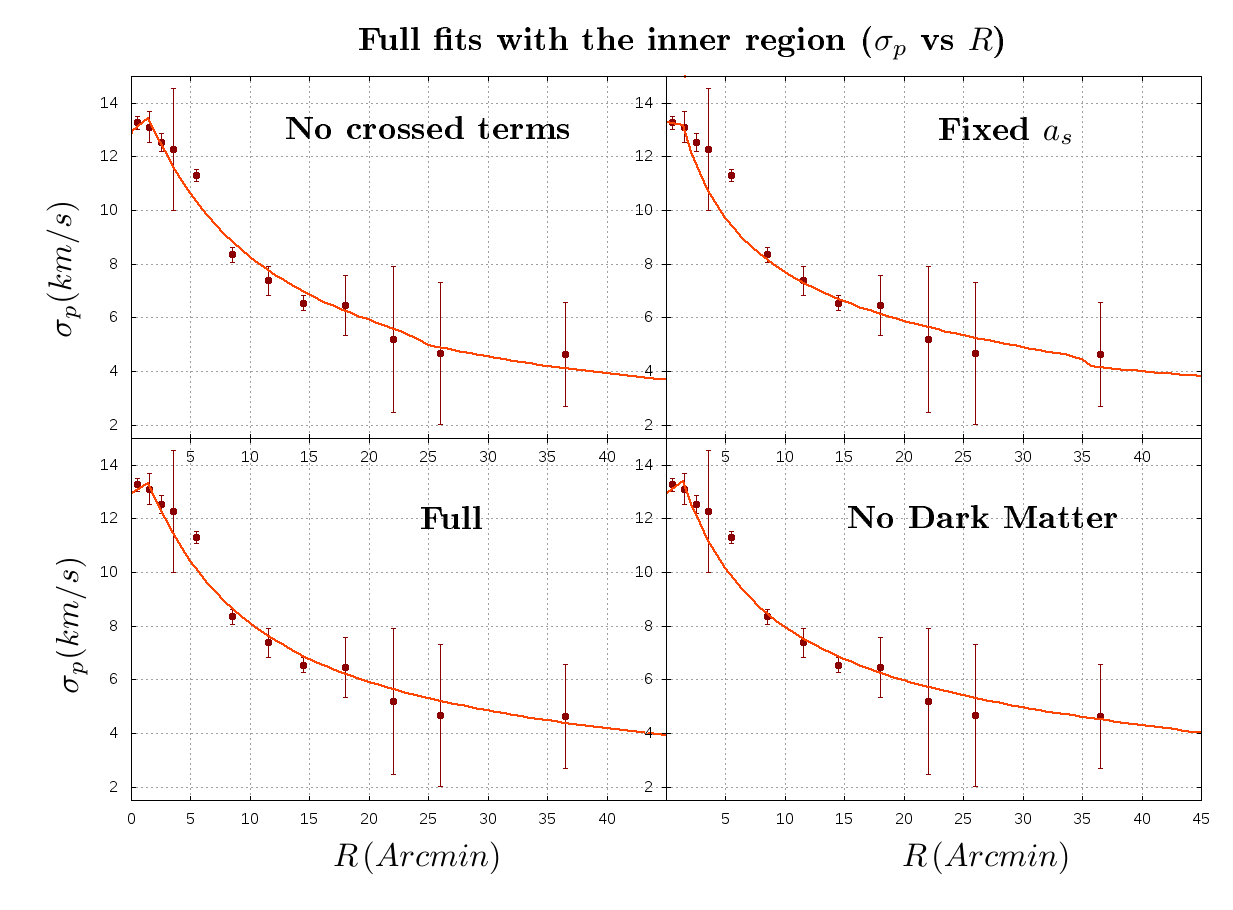
\includegraphics[width=15cm]{images/all_params_refinado_12.png}
\caption[Pg]{Pd}
\end{figure}

\begin{table}[H]
\begin{center}
\begin{tabular}{| c | c | c | c | c | c | c| }
    \hline
    \textbf{Experiment} & $\mathbf{\beta}$ & $\mathbf{a_{dm}} (pc)$ & $\mathbf{a_{s}} (pc)$ & $\mathbf{M_{dm}}$ ($M_{\odot}$) & $\mathbf{M_{s}}$ ($M_{\odot}$) & $\mathbf{\Gamma}$\\ \hline
	No Crossed terms & $0.62$ &	$15.8$ &	$29.0$ &	$5.6 \times 10^{5}$ &	$8.0 \times 10^{4}$ &	$2.2$\\ \hline
	Fix $a_s$ &	$0.0001$ &	$9.0$ &	$2.23$ &	$1.12 \times 10^{5}$ &	$1.06 \times 10 ^{6}$ &	$1.5$\\ \hline
	Full &	$0.46$ &	$15.2$ &	$52.6$ &	$9 \times 10^{5}$ &	$9 \times 10^{5}$ &	$0.38$\\ \hline
	No Dark Matter &	$0.26$ &	$ a = 3.64$ & ----- &	$  M = 1.98 \times 10^{6}$ & ----- & 	$1.24$\\
    \hline
  \end{tabular} 
\caption[It]{Ie}
\end{center}
  
\end{table}

\textbf{All parameters 10}

\begin{figure}[H]
\centering
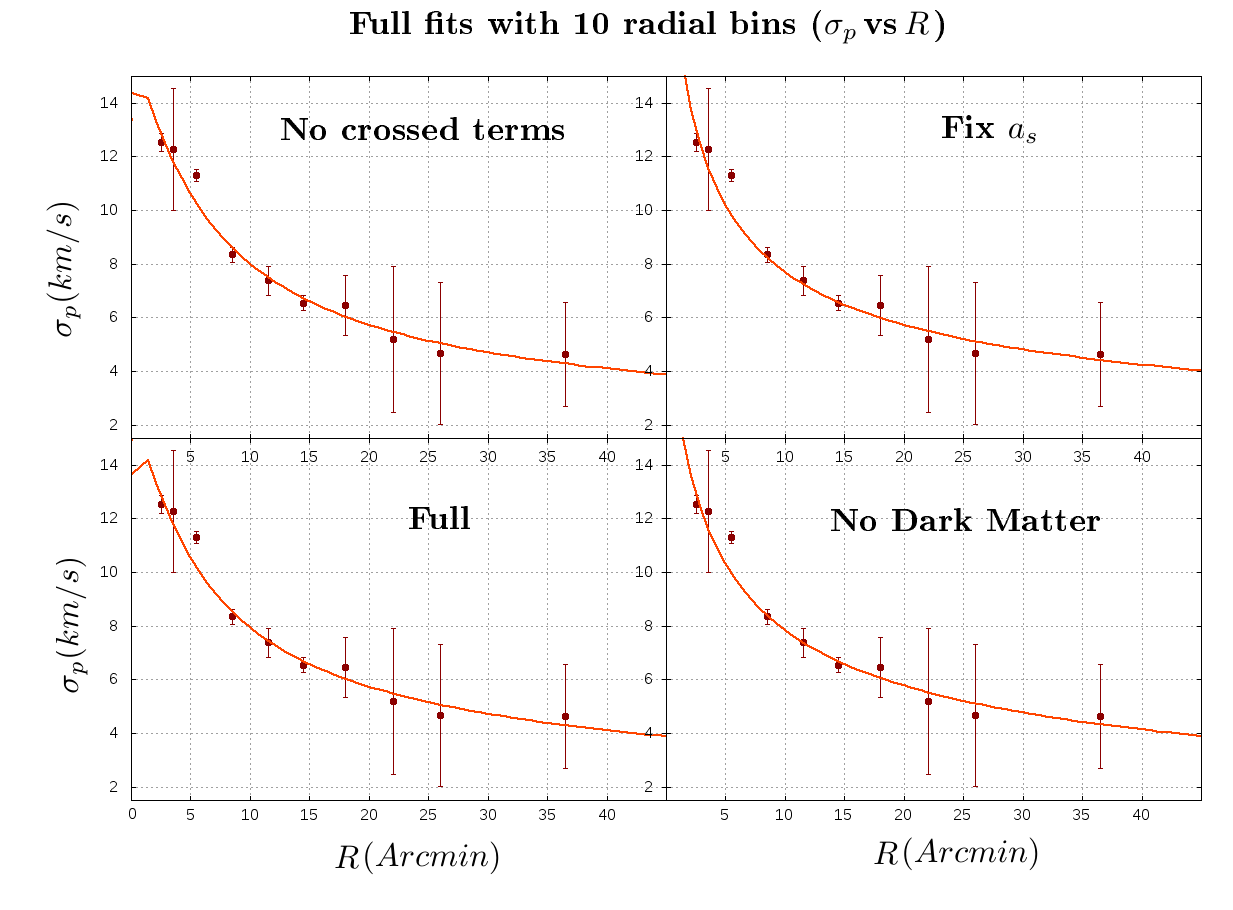
\includegraphics[width=15cm]{images/all_params_refinado_10.png}
\caption[Pg]{Pd}
\end{figure}

\begin{table}[H]
\begin{center}
\begin{tabular}{| c| c| c| c| c| c| c|}
    \hline
    \textbf{Experiment} & $\mathbf{\beta}$ & $\mathbf{a_{dm}} (pc)$ & $\mathbf{a_{s}} (pc)$ & $\mathbf{M_{dm}}$ ($M_{\odot}$) & $\mathbf{M_{s}}$ ($M_{\odot}$) & $\mathbf{\Gamma}$\\ \hline
	No Crossed terms & $0.6$ &	$16$ &	$52.8$ &	$2.1 \times 10^{6}$ &	$2.72 \times 10^{6}$ &	$2.3$\\ \hline
	Fix $a_s$ &	$0.79$ &	$57.9$ &	$2.23$ &	$8 \times 10^{5}$ &	$3.43 \times 10 ^{6}$ &	$2.1$\\ \hline
	Full &	$0.04$ &	$11.8$ &	$57.8$ &	$6 \times 10^{5}$ &	$9 \times 10^{5}$ &	$2.1$\\ \hline
	No Dark Matter &	$0.78$ &	$ a = 2.96$ & ----- &	$  M = 3 \times 10^{6}$ & ----- & 	$1.94$\\
    \hline
  \end{tabular} 
\caption[It]{Ie}
\end{center}
  
\end{table}

\subsection{Fix mass-to-light ratio}

\textbf{Fix mass-to-light ratio 12}

\begin{figure}[H]
\centering
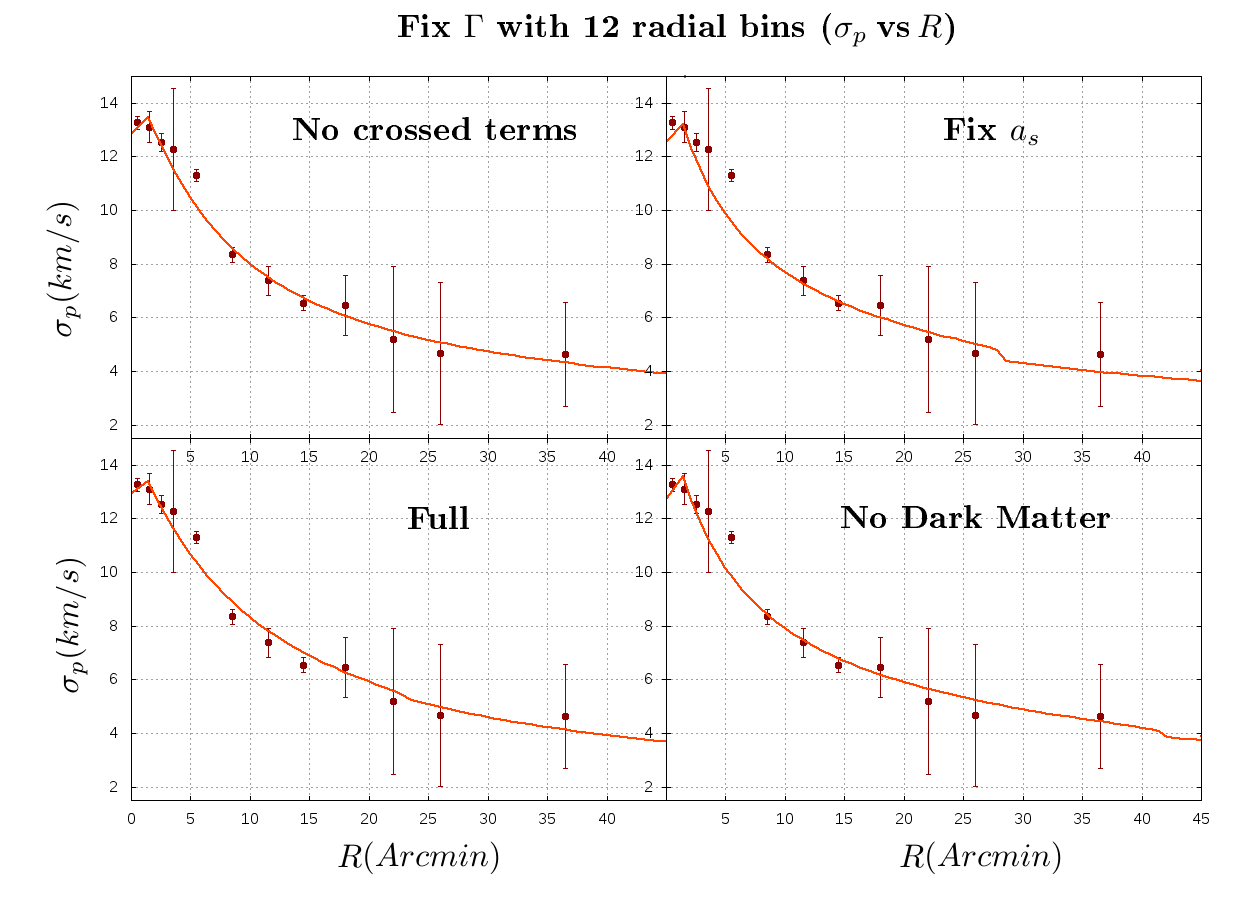
\includegraphics[width=15cm]{images/fix_gamma_refinado_12.png}
\caption[Pg]{Pd}
\end{figure}

\begin{table}[H]
\begin{center}
\begin{tabular}{| c| c| c| c| c| c| c|}
    \hline
    \textbf{Experiment} & $\mathbf{\beta}$ & $\mathbf{a_{dm}} (pc)$ & $\mathbf{a_{s}} (pc)$ & $\mathbf{M_{dm}}$ ($M_{\odot}$) & $\mathbf{M_{s}}$ ($M_{\odot}$) & $\mathbf{\Gamma}$\\ \hline
	No Crossed terms & $0.35$ &	$16.4$ &	$55.62$ &	$1.62 \times 10^{6}$ &	$2.1 \times 10^{6}$ &	$2.5$\\ \hline
	Fix $a_s$ &	$0.001$ &	$3.0$ &	$2.23$ &	$3 \times 10^{5}$ &	$5.0 \times 10 ^{5}$ &	$2.5$\\ \hline
	Full &	$0.72$ &	$20.0$ &	$44.4$ &	$5.2 \times 10^{5}$ &	$8.0 \times 10^{4}$ &	$2.5$\\ \hline
	No Dark Matter &	$0.001$ &	$ a = 3.15$ & ----- &	$  M = 1.52 \times 10^{6}$ & ----- & 	$2.5$\\
    \hline
  \end{tabular} 
\caption[It]{Ie}
\end{center}
  
\end{table}

\textbf{Fix mass-to-light ratio 10}

\begin{figure}[H]
\centering
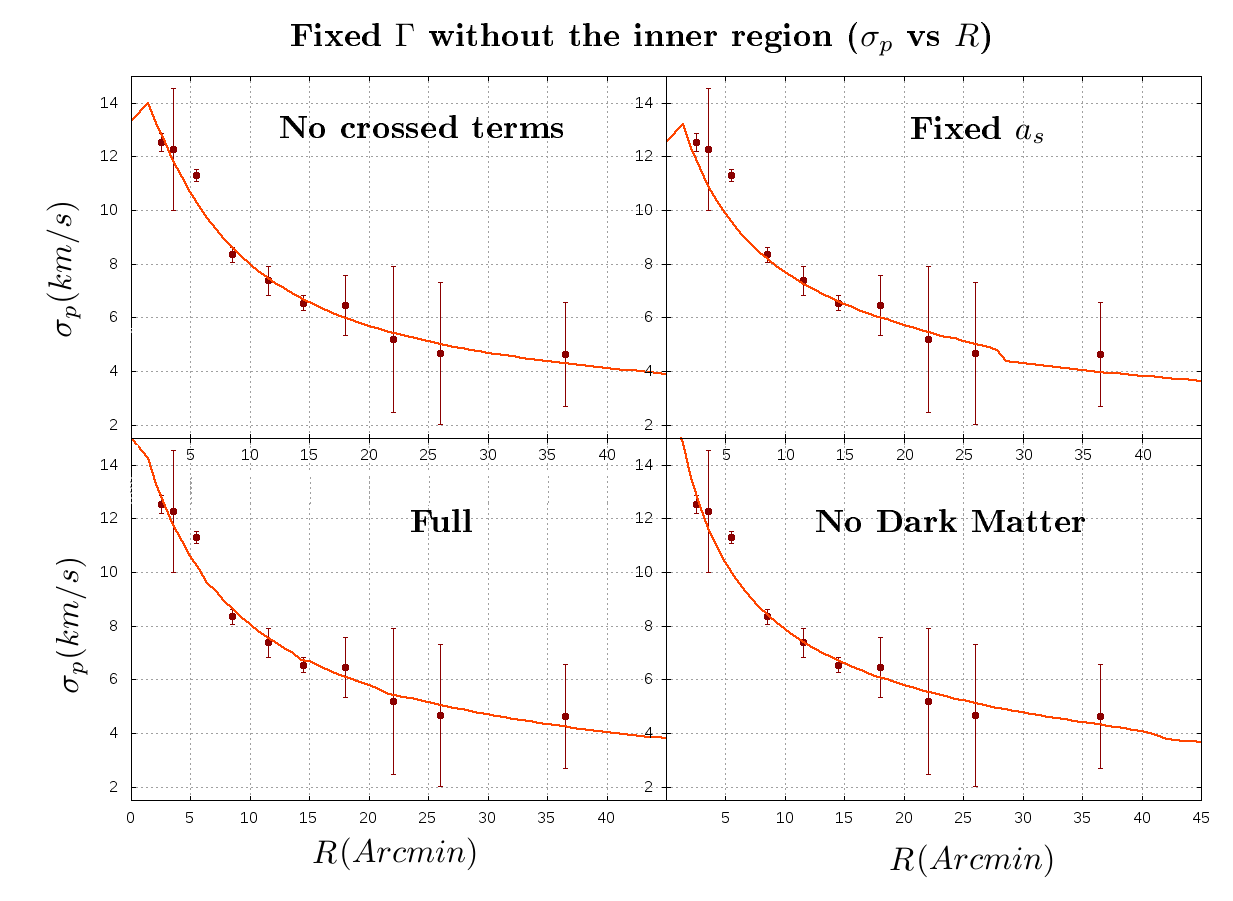
\includegraphics[width=15cm]{images/fix_gamma_refinado_10.png}
\caption[Pg]{Pd}
\end{figure}

\begin{table}[H]
\begin{center}
\begin{tabular}{| c| c| c| c| c| c| c|}
    \hline
    \textbf{Experiment} & $\mathbf{\beta}$ & $\mathbf{a_{dm}} (pc)$ & $\mathbf{a_{s}} (pc)$ & $\mathbf{M_{dm}}$ ($M_{\odot}$) & $\mathbf{M_{s}}$ ($M_{\odot}$) & $\mathbf{\Gamma}$\\ \hline
	No Crossed terms & $0.2$ &	$15.2$ &	$59.8$ &	$1.4 \times 10^{6}$ &	$2.1 \times 10^{6}$ &	$2.5$\\ \hline
	Fix $a_s$ &	$0.801$ &	$3.0$ &	$2.23$ &	$5 \times 10^{5}$ &	$1.0 \times 10 ^{5}$ &	$2.5$\\ \hline
	Full &	$0.9$ &	$16.0$ &	$44.6$ &	$1.62 \times 10^{6}$ &	$1.42 \times 10^{6}$ &	$2.5$\\ \hline
	No Dark Matter &	$0.38$ &	$ a = 2.38$ & ----- &	$  M = 2.03 \times 10^{6}$ & ----- & 	$2.5$\\
    \hline
  \end{tabular} 
\caption[It]{Ie}
\end{center}
  
\end{table}


\section{Stellar Population Synthesis with Starlight}

The stellar mass content of Globular Clusters and Galaxies can be studied through the determination of the stellar populations inside those systems since we have clear knowledge about their photometric properties. If we have information about the amount of stars of a given type inside a stellar system, we can infer how much of the system's mass is given by these populations of stars. 

The determination of the stellar populations can be done using STARLIGHT, which is a Fortran-based program that fits an observed integrated spectrum (Omega Centauri in our case) with a model spectrum which is the sum of $N_{*}$ spectral components from a pre-defined and pre-processed set of base spectra. The program does as many iterations as the user decides to sum up the different template spectra until a good fitting of the spectral lines has been made to the observed spectrum. 

The output of the program after the execution contains the created spectrum (wavelength and intensity) and the approximate percentage of each of the stellar population inside the stellar system. Since the stellar populations are well documented the output will also contain the metallicity of each of them so that further analysis can be made upon STARLIGHT's results.

First, one must prepare the observed spectrum before running STARLIGHT, the spectrum has to be wavelength and flux calibrated, taking into account the bad-pixel removal. Very importantly in the context of mass analysis, the spectrum has to be extinction corrected so that the units of flux relate properly to the units if the templates in STARLIGHT.     

The extinction correction for our observed spectrum is given by

\begin{equation}
f_{obs}(\lambda)=f_{int}(\lambda)10^{-0.4A_{\lambda}}
\end{equation}

Where $A_{\lambda}=0.213$ in the I filter around $8000 \textrm{\AA}$, around the wavelength range of our spectrum. 

On our case, we have to multiply by a factor of 1.216746 the intensity of the spectrum for the flux calibration to be made. After we apply the extinction correction to the spectrum and create an ASCII table with the wavelength, intensity and error columns, it is now ready to be processed with STARLIGHT as we can see in the following figure:

\begin{figure}[H]
\centering
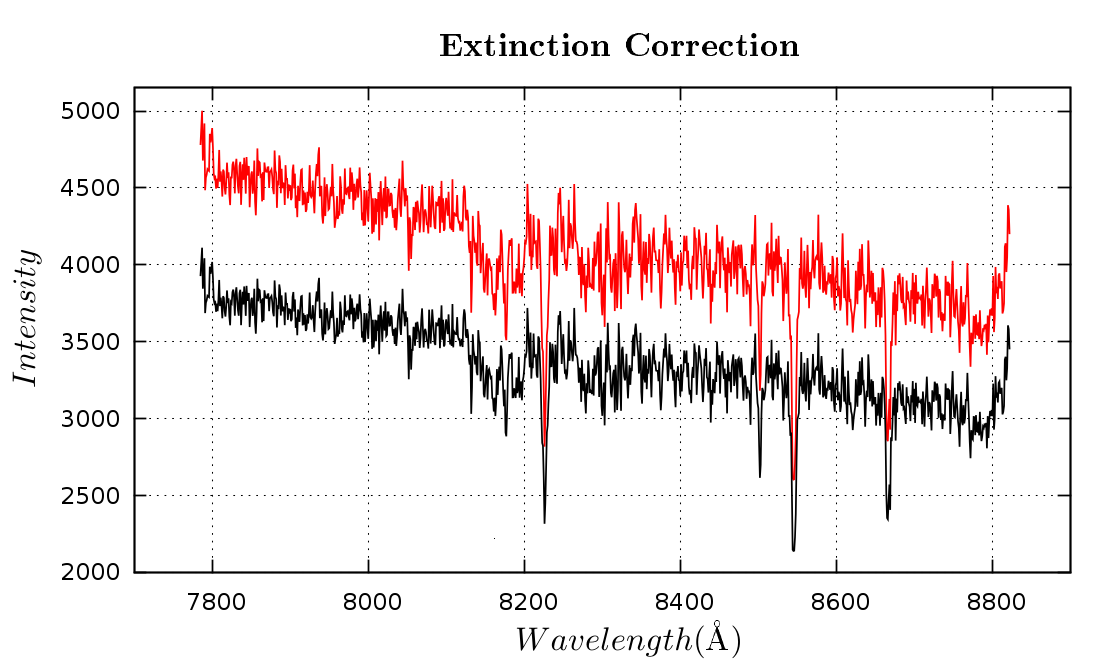
\includegraphics[width=10cm]{images/extinction.png}
\caption[Extinction Correction]{This figure shows an integrated spectrum of the central region of Omega Centauri before and after the extinction correction is applied. The black line has the original flux values and the black line has the corrected flux, that is, the flux that would be observed if there wasn't any interstellar medium that obscures the light coming from the object.}
\end{figure}

Before running STARLIGHT one must assure that the wavelength range is correctly specified in the configuration file that also includes the database of the template spectra and the bad data organized in a mask file. When all of these is ready it is staightforward to run STARLIGHT with the following command:

\begin{center}
./StarlightChains\_v04.exe $<$ Omega\_cen.in
\end{center}

The synthetic spectrum and the original one look like this:

\begin{figure}[H]
\centering
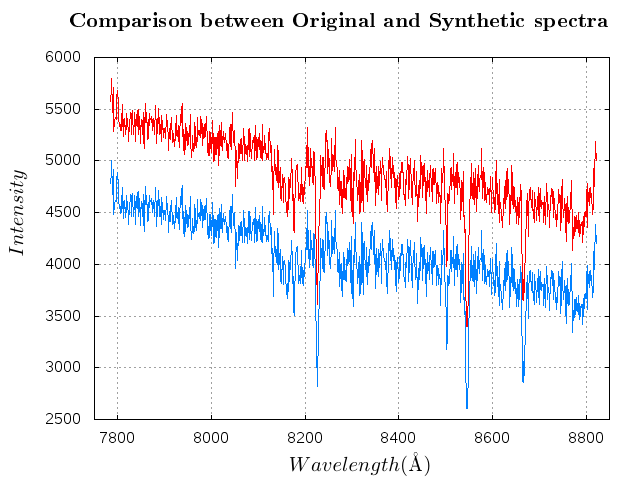
\includegraphics[width=10cm]{images/comparison.png}
\caption[Synthetic spectrum of STARLIGHT]{Synthetic spectrum of Starlight in red, shifted in the y axis for doing the comparison with the original spectrum of Omega Centauri in blue.}
\end{figure}
 
Now, besides the synthetic spectrum, the output file contains some useful results that one can use to calculate the mass of the stellar system. In our case, the relevant parameter that STARLIGHT gives is the stellar mass parameter given by:

\begin{equation}
Mcor\_tot = 3.29446 \times 10^{7}
\end{equation}

And using the formula:

\begin{equation}
M_{s}=Mcor\_tot\times10^{-17}\times4\pi d^{2}\times\left(3.826\times10^{33}\right)^{-1}
\end{equation}

Where $d$ is the luminosity distance in cm, yields a stellar mass of $M_{\star}=243.462M_{\odot}$

This mass is the stellar mass contained in the detection area (that in our set up configuration in OPD ends up to be $A_{D}=0.36\,pc^{2}$) of the integrated spectrum that we analysed with STARLIGHT so if we want to calculate the whole stellar mass of the Globular system we must extrapolate this result to its whole effective area, noting that this will increase the error of the calculation.

If we take the cluster's tidal radius of 40' and it's distance to the sun of $4808.39\,pc$ using a distance modulus of 13.41, then the total effective area (where the stellar mass could be calculated using stellar population synthesis) is $A_{OC}=9833.8\,pc^{2}$. 

Finally, the total stellar mass of the Cluster using this technique can be calculation using:

\begin{equation}
M_{s T} = N \times M_{\star}
\end{equation}

Where N is the number of detection areas within the total effective area of Omega Centauri ($A_{OC}/A_{D}$) of about 31844.8. So that our calculation of the stellar mass is finally:

\begin{equation}
M_{s T} = 6.61 \times 10^{6}M_{\odot}
\end{equation}
 
This result is actually higher than some values  of the dynamical mass found in the literature:

\begin{table}[H]
\begin{center}
\begin{tabular}{| c | c| }
    \hline
    \textbf{Article} & \textbf{Mass} ($M_{\odot}$) \\ \hline
    Mandushev et al. 1991 & $2.4 \times 10^{6}$  \\ \hline
    Pryor \& Meylan & $3.98 \times 10^{6}$  \\ \hline
    Meylan et al. 1995 & $5.1 \times 10^{6}$  \\ \hline
    Majewski et al. 2000 & $5.1 \times 10^{6}$  \\ \hline
    Van de Ven et al. 2006 & $2.5 \times 10^{6}$  \\ \hline
    Cassini et al. 2009 & $3.0 \times 10^{6}$  \\ \hline
    Valcarce \& Catelan, 2011 & $3.0 \times 10^{6}$  \\ \hline
    Jalali et al. 2011 & $2.5 \times 10^{6}$  \\
    \hline
  \end{tabular} 
\caption[Mass Omega Centauri]{Reported values of Omega Centauri's dynamical mass}
\end{center}
\end{table}

The stellar mass should in principle, by smaller or at least equals to the dynamical mass, this discrepancy in our first approach to the mass determination is probably due to errors given by the extrapolation of the results of the detection area to the whole area of the cluster, because our detection area was very small ($\sim 0.2 \, arcmin^{2}$) compared to the cluster's size of more than $6,000 \, arcmin^{2}$. Still, the stellar population technique is consistent with the order of magnitude of the cluster's mass previously reported.  


\begin{figure}[H]
\centering
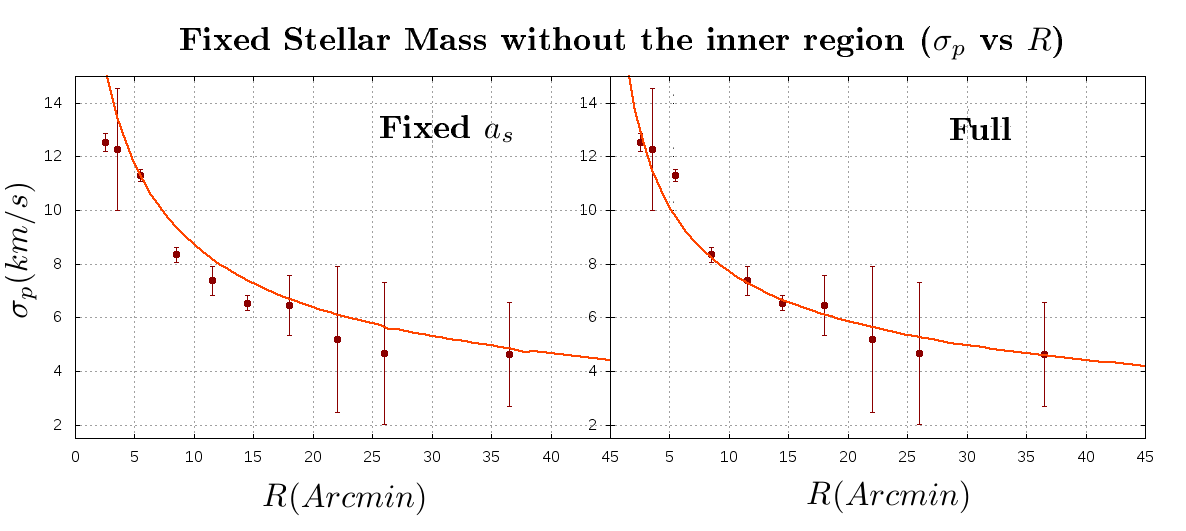
\includegraphics[width=15cm]{images/Starlight_1.png}
\caption[En]{Tt.}
\end{figure}

\begin{table}[H]
\begin{center}
\begin{tabular}{| c| c| c| c| c| c| c|}
    \hline
    \textbf{Experiment} & $\mathbf{\beta}$ & $\mathbf{a_{dm}} (pc)$ & $\mathbf{a_{s}} (pc)$ & $\mathbf{M_{dm}}$ ($M_{\odot}$) & $\mathbf{M_{s}}$ ($M_{\odot}$) & $\mathbf{\Gamma}$\\ \hline
	Fix $a_s$ &	$0.95$ &	$58.0$ &	$2.23$ &	$8 \times 10^{4}$ &	$6.61 \times 10 ^{6}$ &	$2.3$\\ \hline
	Full &	$0.96$ &	$7.36$ &	$50.0$ &	$1.35 \times 10^{6}$ &	$6.61 \times 10^{6}$ &	$1.88$\\ \hline
  \end{tabular} 
\caption[It]{Ie}
\end{center}
  
\end{table}


\begin{figure}[H]
\centering
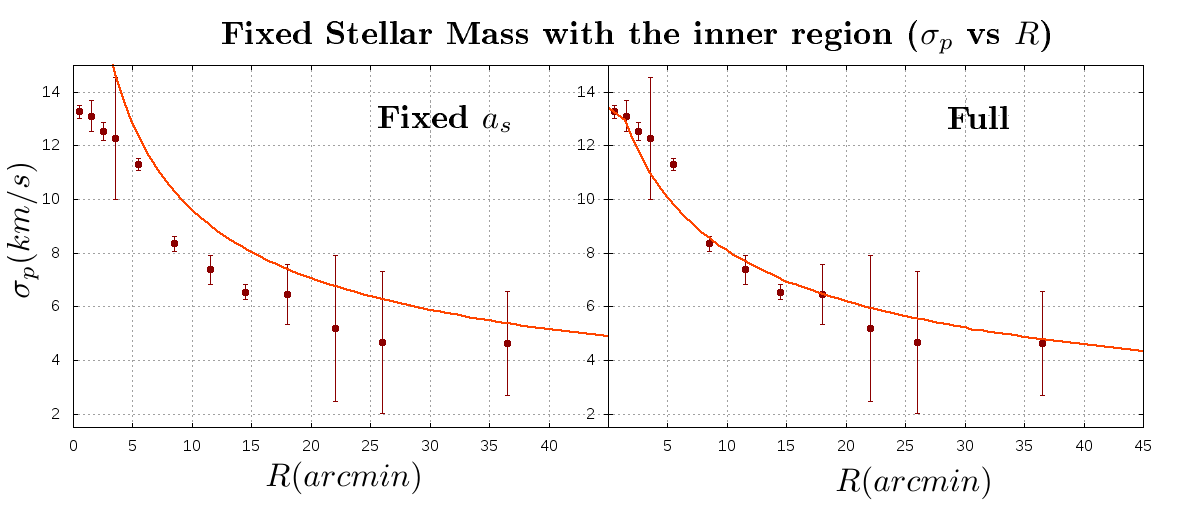
\includegraphics[width=15cm]{images/Starlight_2.png}
\caption[En]{Tct.}
\end{figure}

\begin{table}[H]
\begin{center}
\begin{tabular}{| c| c| c| c| c| c| c|}
    \hline
    \textbf{Experiment} & $\mathbf{\beta}$ & $\mathbf{a_{dm}} (pc)$ & $\mathbf{a_{s}} (pc)$ & $\mathbf{M_{dm}}$ ($M_{\odot}$) & $\mathbf{M_{s}}$ ($M_{\odot}$) & $\mathbf{\Gamma}$\\ \hline
	Fix $a_s$ &	$0.88$ &	$56.98$ &	$2.23$ &	$8 \times 10^{4}$ &	$6.61 \times 10 ^{6}$ &	$1.6$\\ \hline
	Full &	$0.96$ &	$7.6$ &	$12.0$ &	$6.88 \times 10^{5}$ &	$6.61 \times 10^{6}$ &	$0.9$\\ \hline
  \end{tabular} 
\caption[It]{Ie}
\end{center}
  
\end{table} % Modelling

\lhead{\emph{Conclusions}} 
\chapter{Conclusions}

- Cfjsdkafdsjafkl % Conclusions

\begin{thebibliography}{9}
\addcontentsline{toc}{chapter}{Bibliography}


\bibitem{1} 
Michael J. Kurtz, Douglas J. Mink. 
\textit{RVSAO 2.0: Digital Redshifts and Radial Velocities}. 
Harvard-Smithonian Center for Astrophysics, Cambirdge, MA 02138, 1993.

\bibitem{2}
Roueff F., Salati P., Tillet R. 
\textit{The velocity dispersion profile of globular clusters: a closer look}. 
preprint astro-ph/9707174v1.

\bibitem{3} 
Binney J., Tremaine S.. 
\textit{Galactic Dynamics}. 
Princeton University Press, 1994.

\bibitem{4}
http://news.ucsc.edu/2014/11/globular-clusters.html

\bibitem{5}
R. Ibata, C. Nipoti, A. Sollima et. al. 
\textit{Do globular clusters possess Dark Matter halos?}.
MNRAS, Ras 2012.

\bibitem{6}
Joshua J. Adams, Karl Gebhardt, Guillermo A. Blanc et. al. 
\textit{The central Dark Matter distribution of NGC 2976}.
The Astrophysical Journal, 745:92 (17pp), 2012.

\bibitem{7}
P. J. E. Peebles \& R. H. Dicke. 
\textit{Origin of the Globular Star Clusters}.
The Astrophysical Journal, December 1968.

\bibitem{8}
R. G. Gratton, E. Carreta, A. Bragaglia
\textit{Multiple populations in Globular Clusters}.
The Astronomy and Astrophysics Review, 2012.

\bibitem{9}
Richard B. Larson.
\textit{Globular Clusters as Fossils of Galaxy Formation}.
Yale Astronomy Department.

\bibitem{10}
M. E. Sharina, T. H. Puzia, V. L. Afanasiev et. al.
\textit{Globular clusters in low mass galaxies}.
IAU Colloquium No. 198, 2005.

\bibitem{11}
A. Klypin , A. V. Kravtsov et. al. 
\textit{Where Are the Missing Galactic Satellites?} 
The American Astronomical Society, 1999. 

\bibitem{12}
M. Odenkirchen, E. K. Grebel, W. Dehnen et. al.
\textit{The extended tails of palomar 5: A 10$^{\circ}$ Arc of Globular Cluster Tidal Debris}
The American Astronomical Society, 2003.

\bibitem{13}
S. M. Fall \& M. J. Rees.
\textit{A theory for the origin of Globular Clusters}
The Astrophysical Journal, 298: 18-26, 1985.

\bibitem{14}
C. Conroy, A. Loeb \& D. Spergel
\textit{Evidence Against Dark Matter Halos Surrounding the Globular Clusters MGC1 and NGC 2419}
The Astrophysical Journal, October 11$^{th}$ 2009.

\bibitem{15}
S. S. Larse, J. P. Brodie et. al.
\textit{Nitrogen abundances and multiple stellar populations in the Globular Clusters of the Fornax DSPH}
ApJ, accepted (27 Aug 2014).

\bibitem{16}
V. Guglielmo, N. Amoruso, A. Colombo
\textit{Velocity dispersion in Elliptical Galaxies}
The Sky as a laboratory, 2009.

\bibitem{17}
Lars Hernquist
\textit{An analytical model for spherical galaxies and bulges}
ApJ, 356:359-364, 1990 June 20.

\bibitem{18}
URL: \textit{http://www.physics.mcmaster.ca/Globular.html}

\bibitem{19}
Dominici, Tania \& Dos Santos, Claudia Lucia et al. 2008
\textit{Pico dos dias observatory and its instrumentation}
Museu de Astronomia e Ciencias Afins Rio de Janeiro, Brazil, 20921-030

\bibitem{20}
Charbonnel C. et al.
\textit{Are there any first-generation stars in globular clusters today?}
Astronomy \& Astrophysics manuscript no. 2014AA569L6. October 16, 2014.

\bibitem{21}
Portegies Zwart, Simon; McMillan, Stephen L. W.; Gieles, Mark.
\textit{Young Massive Star Clusters}
Annual Review of Astronomy and Astrophysics, vol. 48, p.431-493.

\end{thebibliography}

\label{Bibliography}
\lhead{\emph{Bibliography}}  % Change the left side page header to "Bibliography"
\bibliographystyle{unsrtnat}  % Use the "unsrtnat" BibTeX style for formatting the Bibliography
\bibliography{Bibliography}  % The references (bibliography) information are stored in the file named "Bibliography.bib"

\end{document} 

%% ----------------------------------------------------------------
% Now begin the Appendices, including them as separate files

%\addtocontents{toc}{\vspace{2em}} % Add a gap in the Contents, for aesthetics

%\appendix % Cue to tell LaTeX that the following 'chapters' are Appendices

%\input{Appendices/AppendixA}	% Appendix Title

%\addtocontents{toc}{\vspace{2em}}  % Add a gap in the Contents, for aesthetics
%\backmatter

%% ----------------------------------------------------------------

 % The End
%% ----------------------------------------------------------------